\chapter{Range-clone}
\label{chap:clone}

This chapter describes another \bet operation, range-clone, which can be used
to implement file or directory clones and renames on full-path-indexed \betrfs.
Unlikely a range-rename, which completes all its work at once, a range-clone
injects a new type of message, the \goto messages, to the \bet.
The \bet then flushes \goto messages with other messages in batches, gradually
finishing the range-clone works.
Therefore, range-clone fits into the write-optimized framework of \bets.

This chapter first describes the range-clone interface,
followed by how range-clones are implemented on \bets.
At last, this chapter describes a new technique, preferential splitting, which
makes range-clones more efficient.

\section{The range-clone interface}

\begin{table}[t]
    \centering
    \begin{tabular}{c | l}
        \hline
        Type of File System Operation & Key/Value Store Operations \\
        \hline
        \hline
        File Rename & \mdb$\rightarrow$put(\textit{dst}); \\
                    & \mdb$\rightarrow$del(\textit{src}); \\
                    & \ddb$\rightarrow$range-clone(\textit{src}, \textit{dst}, true); \\
        \hline
        Directory Rename & \mdb$\rightarrow$put(\textit{dst}); \\
                         & \mdb$\rightarrow$del(\textit{src}); \\
                         & \mdb$\rightarrow$range-clone(\textit{src/}, \textit{dst/}, true); \\
                         & \ddb$\rightarrow$range-clone(\textit{src/}, \textit{dst/}, true); \\
        \hline
        File Clone  & \mdb$\rightarrow$put(\textit{dst}); \\
                    & \ddb$\rightarrow$range-clone(\textit{src}, \textit{dst}, false); \\
        \hline
        Directory Clone  & \mdb$\rightarrow$put(\textit{dst}); \\
                         & \mdb$\rightarrow$range-clone(\textit{src/}, \textit{dst/}, false); \\
                         & \ddb$\rightarrow$range-clone(\textit{src/}, \textit{dst/}, false); \\
        \hline
    \end{tabular}
    \caption[File system renames and clones in \betrfs with range-clones]{\label{tab:fsrc}
        \betrfs renames or clones \textit{src} to \textit{dst} by calling range-clones.}
\end{table}

Similar to range-rename, range-clone is defined as:
range-clone(\spre, \dpre, \delold), where \delold is a boolean.
It does the following things:
\begin{itemize}
\item it deletes all destination key/value pairs from the key/value store;
\item then, for any source key/value pair $(k,v)$ in the key/value store,
it inserts a key/value pair $(k',v)$ to the key/value store,
where $k$ is the concatenation of \spre and some suffix $s$ and $k'$ is the
concatenation of \dpre and the same suffix $s$;
\item if \delold is true, it deletes all source key/value pairs from the
key/value store.
\end{itemize}
If \delold is true, range-clone is equivalent to range-rename;
otherwise, range-clone is range-rename without deleting source key/value pairs.
Therefore, as summarized in Table~\ref{tab:fsrc},
file or directory renames on full-path-indexed \betrfs can be done
with range-clones just as they are done with range-renames.
And clones on full-path-index \betrfs are done in the similar ways with \delold
set to false.

\section{The range-clone operation}

This section shows the implementation of range-clone operations.
Because deleting source key/value pairs can be done by injecting a range-delete
message into the root node,
\delold is set to false throughout the section.

This section first shows all the changes needed if performing all operations
at the time of the range-clone, that is, all operations are on the critical
path, and mutual exclusion on the tree.
Then, this section shows how to enhance the design to minimize the critical
path, reduce locking, and move as much work as possible to the background.
Moving work to the background also reduce the total amount of CPU and IO work,
since \bets are designed to buffer changes and to schedule them IO-efficiently.

\subsection{Range-clone, on the critical path}

\begin{figure}
    \begin{subfigure}{\textwidth}
        \centering
        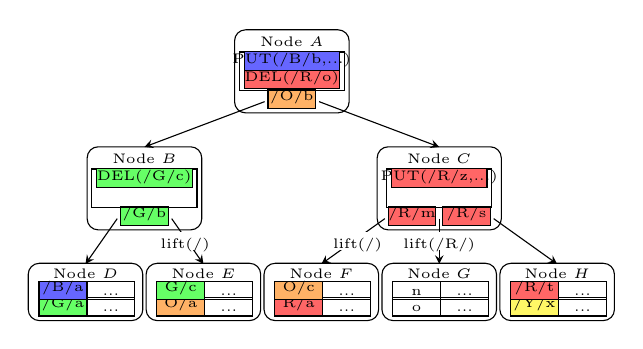
\begin{tikzpicture}[xscale=0.95, yscale=0.95]
            \node[anchor=south, rectangle, rounded corners, minimum height=.06\textwidth, minimum width=.12\textwidth, draw=black] at (0, 0) {};
            \node[anchor=south, font=\tiny] at (0, .036\textwidth) {Node $F$};
            \node[anchor=south, rectangle, minimum height=.015\textwidth, minimum width=.05\textwidth, draw=black, fill={red!60}] at (-.025\textwidth, .005\textwidth) {};
            \node[anchor=south, font=\tiny] at (-.025\textwidth, 0) {R/a};
            \node[anchor=south, rectangle, minimum height=.015\textwidth, minimum width=.05\textwidth, draw=black] at (.028\textwidth, .005\textwidth) {};
            \node[anchor=south, font=\tiny] at (.028\textwidth, 0) {...};
            \node[anchor=south, rectangle, minimum height=.015\textwidth, minimum width=.05\textwidth, draw=black, fill={orange!60}] at (-.025\textwidth, .023\textwidth) {};
            \node[anchor=south, font=\tiny] at (-.025\textwidth, .018\textwidth) {O/c};
            \node[anchor=south, rectangle, minimum height=.015\textwidth, minimum width=.05\textwidth, draw=black] at (.028\textwidth, .023\textwidth) {};
            \node[anchor=south, font=\tiny] at (.028\textwidth, .018\textwidth) {...};

            \node[anchor=south, rectangle, rounded corners, minimum height=.06\textwidth, minimum width=.12\textwidth, draw=black] at (.13\textwidth, 0) {};
            \node[anchor=south, font=\tiny] at (.13\textwidth, .036\textwidth) {Node $G$};
            \node[anchor=south, rectangle, minimum height=.015\textwidth, minimum width=.05\textwidth, draw=black] at (.105\textwidth, .005\textwidth) {};
            \node[anchor=south, font=\tiny] at (.105\textwidth, 0) {o};
            \node[anchor=south, rectangle, minimum height=.015\textwidth, minimum width=.05\textwidth, draw=black] at (.158\textwidth, .005\textwidth) {};
            \node[anchor=south, font=\tiny] at (.158\textwidth, 0) {...};
            \node[anchor=south, rectangle, minimum height=.015\textwidth, minimum width=.05\textwidth, draw=black] at (.105\textwidth, .023\textwidth) {};
            \node[anchor=south, font=\tiny] at (.105\textwidth, .018\textwidth) {n};
            \node[anchor=south, rectangle, minimum height=.015\textwidth, minimum width=.05\textwidth, draw=black] at (.158\textwidth, .023\textwidth) {};
            \node[anchor=south, font=\tiny] at (.158\textwidth, .018\textwidth) {...};

            \node[anchor=south, rectangle, rounded corners, minimum height=.06\textwidth, minimum width=.12\textwidth, draw=black] at (.26\textwidth, 0) {};
            \node[anchor=south, font=\tiny] at (.26\textwidth, .036\textwidth) {Node $H$};
            \node[anchor=south, rectangle, minimum height=.015\textwidth, minimum width=.05\textwidth, draw=black, fill={yellow!60}] at (.235\textwidth, .005\textwidth) {};
            \node[anchor=south, font=\tiny] at (.235\textwidth, 0) {/Y/x};
            \node[anchor=south, rectangle, minimum height=.015\textwidth, minimum width=.05\textwidth, draw=black] at (.288\textwidth, .005\textwidth) {};
            \node[anchor=south, font=\tiny] at (.288\textwidth, 0) {...};
            \node[anchor=south, rectangle, minimum height=.015\textwidth, minimum width=.05\textwidth, draw=black, fill={red!60}] at (.235\textwidth, .023\textwidth) {};
            \node[anchor=south, font=\tiny] at (.235\textwidth, .018\textwidth) {/R/t};
            \node[anchor=south, rectangle, minimum height=.015\textwidth, minimum width=.05\textwidth, draw=black] at (.288\textwidth, .023\textwidth) {};
            \node[anchor=south, font=\tiny] at (.288\textwidth, .018\textwidth) {...};

            \node[anchor=south, rectangle, rounded corners, minimum height=.06\textwidth, minimum width=.12\textwidth, draw=black] at (-.13\textwidth, 0) {};
            \node[anchor=south, font=\tiny] at (-.13\textwidth, .036\textwidth) {Node $E$};
            \node[anchor=south, rectangle, minimum height=.015\textwidth, minimum width=.05\textwidth, draw=black, fill={orange!60}] at (-.155\textwidth, .005\textwidth) {};
            \node[anchor=south, font=\tiny] at (-.155\textwidth, 0) {O/a};
            \node[anchor=south, rectangle, minimum height=.015\textwidth, minimum width=.05\textwidth, draw=black] at (-.102\textwidth, .005\textwidth) {};
            \node[anchor=south, font=\tiny] at (-.102\textwidth, 0) {...};
            \node[anchor=south, rectangle, minimum height=.015\textwidth, minimum width=.05\textwidth, draw=black, fill={green!60}] at (-.155\textwidth, .023\textwidth) {};
            \node[anchor=south, font=\tiny] at (-.155\textwidth, .018\textwidth) {G/c};
            \node[anchor=south, rectangle, minimum height=.015\textwidth, minimum width=.05\textwidth, draw=black] at (-.102\textwidth, .023\textwidth) {};
            \node[anchor=south, font=\tiny] at (-.102\textwidth, .018\textwidth) {...};

            \node[anchor=south, rectangle, rounded corners, minimum height=.06\textwidth, minimum width=.12\textwidth, draw=black] at (-.26\textwidth, 0) {};
            \node[anchor=south, font=\tiny] at (-.26\textwidth, .036\textwidth) {Node $D$};
            \node[anchor=south, rectangle, minimum height=.015\textwidth, minimum width=.05\textwidth, draw=black, fill={green!60}] at (-.285\textwidth, .005\textwidth) {};
            \node[anchor=south, font=\tiny] at (-.285\textwidth, 0) {/G/a};
            \node[anchor=south, rectangle, minimum height=.015\textwidth, minimum width=.05\textwidth, draw=black] at (-.232\textwidth, .005\textwidth) {};
            \node[anchor=south, font=\tiny] at (-.232\textwidth, 0) {...};
            \node[anchor=south, rectangle, minimum height=.015\textwidth, minimum width=.05\textwidth, draw=black, fill={blue!60}] at (-.285\textwidth, .023\textwidth) {};
            \node[anchor=south, font=\tiny] at (-.285\textwidth, .018\textwidth) {/B/a};
            \node[anchor=south, rectangle, minimum height=.015\textwidth, minimum width=.05\textwidth, draw=black] at (-.232\textwidth, .023\textwidth) {};
            \node[anchor=south, font=\tiny] at (-.232\textwidth, .018\textwidth) {...};

            \node[anchor=south, rectangle, rounded corners, minimum height=.087\textwidth, minimum width=.12\textwidth, draw=black] at (-.195\textwidth, .1\textwidth) {};
            \node[anchor=south, font=\tiny] at (-.195\textwidth, .163\textwidth) {Node $B$};
            \node[anchor=south, rectangle, minimum height=.015\textwidth, minimum width=.05\textwidth, draw=black, fill={green!60}] at (-.195\textwidth, .105\textwidth) {};
            \node[anchor=south, font=\tiny] at (-.195\textwidth, .1\textwidth) {/G/b};
            \node[anchor=south, rectangle, minimum height=.04\textwidth, minimum width=.11\textwidth, draw=black] at (-.195\textwidth, .125\textwidth) {};
            \node[anchor=south, rectangle, minimum height=.015\textwidth, minimum width=.1\textwidth, draw=black, fill={green!60}] at (-.195\textwidth, .147\textwidth) {};
            \node[anchor=south, font=\tiny] at  (-.195\textwidth, .141\textwidth) {DEL(/G/c)};

            \node[anchor=south, rectangle, rounded corners, minimum height=.087\textwidth, minimum width=.13\textwidth, draw=black] at (.13\textwidth, .1\textwidth) {};
            \node[anchor=south, font=\tiny] at (.13\textwidth, .163\textwidth) {Node $C$};
            \node[anchor=south, rectangle, minimum height=.015\textwidth, minimum width=.05\textwidth, draw=black, fill={red!60}] at (.1\textwidth, .105\textwidth) {};
            \node[anchor=south, font=\tiny] at (.1\textwidth, .1\textwidth) {/R/m};
            \node[anchor=south, rectangle, minimum height=.015\textwidth, minimum width=.05\textwidth, draw=black, fill={red!60}] at (.16\textwidth, .105\textwidth) {};
            \node[anchor=south, font=\tiny] at (.16\textwidth, .1\textwidth) {/R/s};
            \node[anchor=south, rectangle, minimum height=.04\textwidth, minimum width=.11\textwidth, draw=black] at (.13\textwidth, .125\textwidth) {};
            \node[anchor=south, rectangle, minimum height=.015\textwidth, minimum width=.1\textwidth, draw=black, fill={red!60}] at (.13\textwidth, .147\textwidth) {};
            \node[anchor=south, font=\tiny] at  (.13\textwidth, .141\textwidth) {PUT(/R/z,...)};

            \node[anchor=south, rectangle, rounded corners, minimum height=.087\textwidth, minimum width=.12\textwidth, draw=black] at (-.0325\textwidth, .229\textwidth) {};
            \node[anchor=south, font=\tiny] at (-.0325\textwidth, .292\textwidth) {Node $A$};
            \node[anchor=south, rectangle, minimum height=.015\textwidth, minimum width=.05\textwidth, draw=black, fill={orange!60}] at (-.0325\textwidth, .234\textwidth) {};
            \node[anchor=south, font=\tiny] at (-.0325\textwidth, .229\textwidth) {/O/b};
            \node[anchor=south, rectangle, minimum height=.04\textwidth, minimum width=.11\textwidth, draw=black] at (-.0325\textwidth, .254\textwidth) {};
            \node[anchor=south, rectangle, minimum height=.015\textwidth, minimum width=.1\textwidth, draw=black, fill={red!60}] at (-.0325\textwidth, .256\textwidth) {};
            \node[anchor=south, font=\tiny] at  (-.0325\textwidth, .25\textwidth) {DEL(/R/o)};
            \node[anchor=south, rectangle, minimum height=.015\textwidth, minimum width=.1\textwidth, draw=black, fill={blue!60}] at (-.0325\textwidth, .276\textwidth) {};
            \node[anchor=south, font=\tiny] at  (-.0325\textwidth, .27\textwidth) {PUT(/B/b,...)};

            \draw[->, >=stealth] (-.225\textwidth, .113\textwidth) -- (-.26\textwidth, .063\textwidth);
            \draw[->, >=stealth] (-.165\textwidth, .113\textwidth) -- (-.13\textwidth, .063\textwidth);
            \draw[->, >=stealth] (.13\textwidth, .113\textwidth) -- (.13\textwidth, .063\textwidth);
            \draw[->, >=stealth] (.19\textwidth, .113\textwidth) -- (.26\textwidth, .063\textwidth);
            \draw[->, >=stealth] (.07\textwidth, .113\textwidth) -- (0, .063\textwidth);
            \draw[->, >=stealth] (-.0625\textwidth, .242\textwidth) -- (-.195\textwidth, .192\textwidth);
            \draw[->, >=stealth] (-.0025\textwidth, .242\textwidth) -- (.13\textwidth, .192\textwidth);

            \node[anchor=north,rectangle, minimum height=.015\textwidth, minimum width=.05\textwidth, fill={white}] at (.13\textwidth, .099\textwidth) {};
            \node[anchor=north, font=\tiny] at (.13\textwidth, .102\textwidth) {lift(/R/)};
            \node[anchor=north,rectangle, minimum height=.015\textwidth, minimum width=.05\textwidth, fill={white}] at (.04\textwidth, .099\textwidth) {};
            \node[anchor=north, font=\tiny] at (.04\textwidth, .102\textwidth) {lift(/)};
            \node[anchor=north,rectangle, minimum height=.015\textwidth, minimum width=.05\textwidth, fill={white}] at (-.15\textwidth, .099\textwidth) {};
            \node[anchor=north, font=\tiny] at (-.15\textwidth, .102\textwidth) {lift(/)};
        \end{tikzpicture}
        \caption{\label{subfig:rc-1} The \bet before the range-clone.}
    \end{subfigure}
    \begin{subfigure}{\textwidth}
        \centering
        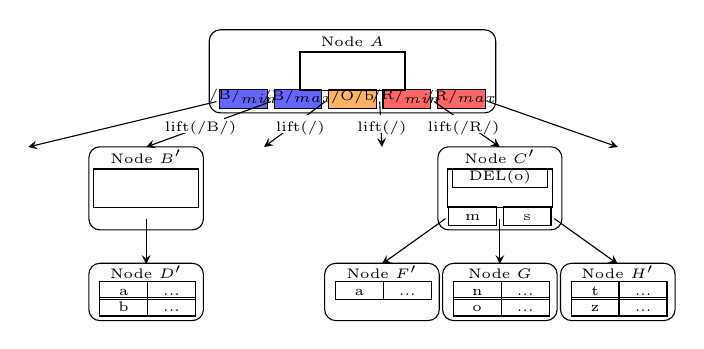
\begin{tikzpicture}[xscale=0.95, yscale=0.95]
            \node[anchor=south, rectangle, rounded corners, minimum height=.06\textwidth, minimum width=.12\textwidth, draw=black] at (0, 0) {};
            \node[anchor=south, font=\tiny] at (0, .036\textwidth) {Node $F'$};
            \node[anchor=south, rectangle, minimum height=.015\textwidth, minimum width=.05\textwidth, draw=black] at (-.025\textwidth, .023\textwidth) {};
            \node[anchor=south, font=\tiny] at (-.025\textwidth, .018\textwidth) {a};
            \node[anchor=south, rectangle, minimum height=.015\textwidth, minimum width=.05\textwidth, draw=black] at (.028\textwidth, .023\textwidth) {};
            \node[anchor=south, font=\tiny] at (.028\textwidth, .018\textwidth) {...};

            \node[anchor=south, rectangle, rounded corners, minimum height=.06\textwidth, minimum width=.12\textwidth, draw=black] at (.13\textwidth, 0) {};
            \node[anchor=south, font=\tiny] at (.13\textwidth, .036\textwidth) {Node $G$};
            \node[anchor=south, rectangle, minimum height=.015\textwidth, minimum width=.05\textwidth, draw=black] at (.105\textwidth, .005\textwidth) {};
            \node[anchor=south, font=\tiny] at (.105\textwidth, 0) {o};
            \node[anchor=south, rectangle, minimum height=.015\textwidth, minimum width=.05\textwidth, draw=black] at (.158\textwidth, .005\textwidth) {};
            \node[anchor=south, font=\tiny] at (.158\textwidth, 0) {...};
            \node[anchor=south, rectangle, minimum height=.015\textwidth, minimum width=.05\textwidth, draw=black] at (.105\textwidth, .023\textwidth) {};
            \node[anchor=south, font=\tiny] at (.105\textwidth, .018\textwidth) {n};
            \node[anchor=south, rectangle, minimum height=.015\textwidth, minimum width=.05\textwidth, draw=black] at (.158\textwidth, .023\textwidth) {};
            \node[anchor=south, font=\tiny] at (.158\textwidth, .018\textwidth) {...};

            \node[anchor=south, rectangle, rounded corners, minimum height=.06\textwidth, minimum width=.12\textwidth, draw=black] at (.26\textwidth, 0) {};
            \node[anchor=south, font=\tiny] at (.26\textwidth, .036\textwidth) {Node $H'$};
            \node[anchor=south, rectangle, minimum height=.015\textwidth, minimum width=.05\textwidth, draw=black] at (.235\textwidth, .005\textwidth) {};
            \node[anchor=south, font=\tiny] at (.235\textwidth, 0) {z};
            \node[anchor=south, rectangle, minimum height=.015\textwidth, minimum width=.05\textwidth, draw=black] at (.288\textwidth, .005\textwidth) {};
            \node[anchor=south, font=\tiny] at (.288\textwidth, 0) {...};
            \node[anchor=south, rectangle, minimum height=.015\textwidth, minimum width=.05\textwidth, draw=black] at (.235\textwidth, .023\textwidth) {};
            \node[anchor=south, font=\tiny] at (.235\textwidth, .018\textwidth) {t};
            \node[anchor=south, rectangle, minimum height=.015\textwidth, minimum width=.05\textwidth, draw=black] at (.288\textwidth, .023\textwidth) {};
            \node[anchor=south, font=\tiny] at (.288\textwidth, .018\textwidth) {...};

            \node[anchor=south, rectangle, rounded corners, minimum height=.06\textwidth, minimum width=.12\textwidth, draw=black] at (-.26\textwidth, 0) {};
            \node[anchor=south, font=\tiny] at (-.26\textwidth, .036\textwidth) {Node $D'$};
            \node[anchor=south, rectangle, minimum height=.015\textwidth, minimum width=.05\textwidth, draw=black] at (-.285\textwidth, .005\textwidth) {};
            \node[anchor=south, font=\tiny] at (-.285\textwidth, 0) {b};
            \node[anchor=south, rectangle, minimum height=.015\textwidth, minimum width=.05\textwidth, draw=black] at (-.232\textwidth, .005\textwidth) {};
            \node[anchor=south, font=\tiny] at (-.232\textwidth, 0) {...};
            \node[anchor=south, rectangle, minimum height=.015\textwidth, minimum width=.05\textwidth, draw=black] at (-.285\textwidth, .023\textwidth) {};
            \node[anchor=south, font=\tiny] at (-.285\textwidth, .018\textwidth) {a};
            \node[anchor=south, rectangle, minimum height=.015\textwidth, minimum width=.05\textwidth, draw=black] at (-.232\textwidth, .023\textwidth) {};
            \node[anchor=south, font=\tiny] at (-.232\textwidth, .018\textwidth) {...};

            \node[anchor=south, rectangle, rounded corners, minimum height=.087\textwidth, minimum width=.12\textwidth, draw=black] at (-.26\textwidth, .1\textwidth) {};
            \node[anchor=south, font=\tiny] at (-.26\textwidth, .163\textwidth) {Node $B'$};
            \node[anchor=south, rectangle, minimum height=.04\textwidth, minimum width=.11\textwidth, draw=black] at (-.26\textwidth, .125\textwidth) {};

            \node[anchor=south, rectangle, rounded corners, minimum height=.087\textwidth, minimum width=.13\textwidth, draw=black] at (.13\textwidth, .1\textwidth) {};
            \node[anchor=south, font=\tiny] at (.13\textwidth, .163\textwidth) {Node $C'$};
            \node[anchor=south, rectangle, minimum height=.015\textwidth, minimum width=.05\textwidth, draw=black] at (.1\textwidth, .105\textwidth) {};
            \node[anchor=south, font=\tiny] at (.1\textwidth, .1\textwidth) {m};
            \node[anchor=south, rectangle, minimum height=.015\textwidth, minimum width=.05\textwidth, draw=black] at (.16\textwidth, .105\textwidth) {};
            \node[anchor=south, font=\tiny] at (.16\textwidth, .1\textwidth) {s};
            \node[anchor=south, rectangle, minimum height=.04\textwidth, minimum width=.11\textwidth, draw=black] at (.13\textwidth, .125\textwidth) {};
            \node[anchor=south, rectangle, minimum height=.015\textwidth, minimum width=.1\textwidth, draw=black] at (.13\textwidth, .147\textwidth) {};
            \node[anchor=south, font=\tiny] at  (.13\textwidth, .141\textwidth) {DEL(o)};

            \node[anchor=south, rectangle, rounded corners, minimum height=.087\textwidth, minimum width=.3\textwidth, draw=black] at (-.0325\textwidth, .229\textwidth) {};
            \node[anchor=south, font=\tiny] at (-.0325\textwidth, .292\textwidth) {Node $A$};
            \node[anchor=south, rectangle, minimum height=.015\textwidth, minimum width=.05\textwidth, draw=black, fill={blue!60}] at (-.1525\textwidth, .234\textwidth) {};
            \node[anchor=south, font=\tiny] at (-.1525\textwidth, .229\textwidth) {/B/$_{min}$};
            \node[anchor=south, rectangle, minimum height=.015\textwidth, minimum width=.05\textwidth, draw=black, fill={blue!60}] at (-.0925\textwidth, .234\textwidth) {};
            \node[anchor=south, font=\tiny] at (-.0925\textwidth, .229\textwidth) {/B/$_{max}$};
            \node[anchor=south, rectangle, minimum height=.015\textwidth, minimum width=.05\textwidth, draw=black, fill={orange!60}] at (-.0325\textwidth, .234\textwidth) {};
            \node[anchor=south, font=\tiny] at (-.0325\textwidth, .229\textwidth) {/O/b};
            \node[anchor=south, rectangle, minimum height=.015\textwidth, minimum width=.05\textwidth, draw=black, fill={red!60}] at (.0275\textwidth, .234\textwidth) {};
            \node[anchor=south, font=\tiny] at (.0275\textwidth, .229\textwidth) {/R/$_{min}$};
            \node[anchor=south, rectangle, minimum height=.015\textwidth, minimum width=.05\textwidth, draw=black, fill={red!60}] at (.0875\textwidth, .234\textwidth) {};
            \node[anchor=south, font=\tiny] at (.0875\textwidth, .229\textwidth) {/R/$_{max}$};
            \node[anchor=south, rectangle, minimum height=.04\textwidth, minimum width=.11\textwidth, draw=black] at (-.0325\textwidth, .254\textwidth) {};

            \draw[->, >=stealth] (-.26\textwidth, .113\textwidth) -- (-.26\textwidth, .063\textwidth);
            \draw[->, >=stealth] (.13\textwidth, .113\textwidth) -- (.13\textwidth, .063\textwidth);
            \draw[->, >=stealth] (.19\textwidth, .113\textwidth) -- (.26\textwidth, .063\textwidth);
            \draw[->, >=stealth] (.07\textwidth, .113\textwidth) -- (0, .063\textwidth);
            \draw[->, >=stealth] (-.1825\textwidth, .242\textwidth) -- (-.39\textwidth, .192\textwidth);
            \draw[->, >=stealth] (-.1225\textwidth, .242\textwidth) -- (-.26\textwidth, .192\textwidth);
            \draw[->, >=stealth] (-.0625\textwidth, .242\textwidth) -- (-.13\textwidth, .192\textwidth);
            \draw[->, >=stealth] (-.0025\textwidth, .242\textwidth) -- (0, .192\textwidth);
            \draw[->, >=stealth] (.0575\textwidth, .242\textwidth) -- (.13\textwidth, .192\textwidth);
            \draw[->, >=stealth] (.1175\textwidth, .242\textwidth) -- (.26\textwidth, .192\textwidth);

            \node[anchor=north,rectangle, minimum height=.015\textwidth, minimum width=.05\textwidth, fill={white}] at (-.20\textwidth, .228\textwidth) {};
            \node[anchor=north, font=\tiny] at (-.20\textwidth, .231\textwidth) {lift(/B/)};
            \node[anchor=north,rectangle, minimum height=.015\textwidth, minimum width=.05\textwidth, fill={white}] at (-.09\textwidth, .228\textwidth) {};
            \node[anchor=north, font=\tiny] at (-.09\textwidth, .231\textwidth) {lift(/)};
            \node[anchor=north,rectangle, minimum height=.015\textwidth, minimum width=.05\textwidth, fill={white}] at (0, .228\textwidth) {};
            \node[anchor=north, font=\tiny] at (0, .231\textwidth) {lift(/)};
            \node[anchor=north,rectangle, minimum height=.015\textwidth, minimum width=.05\textwidth, fill={white}] at (.09\textwidth, .228\textwidth) {};
            \node[anchor=north, font=\tiny] at (.09\textwidth, .231\textwidth) {lift(/R/)};
        \end{tikzpicture}
        \caption{\label{subfig:rc-2} The range-clone slices out the source and
            destination subtrees.}
    \end{subfigure}
    \begin{subfigure}{\textwidth}
        \centering
        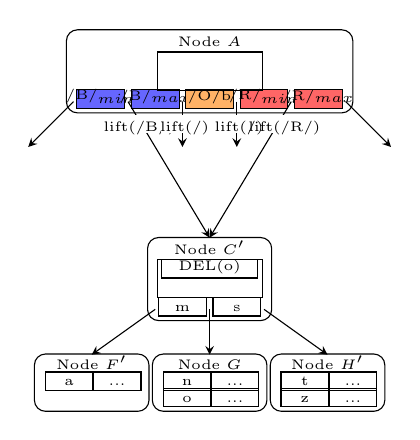
\begin{tikzpicture}[xscale=0.95, yscale=0.95]
            \node[anchor=south, rectangle, rounded corners, minimum height=.06\textwidth, minimum width=.12\textwidth, draw=black] at (-.1625\textwidth, -.1\textwidth) {};
            \node[anchor=south, font=\tiny] at (-.1625\textwidth, -.064\textwidth) {Node $F'$};
            \node[anchor=south, rectangle, minimum height=.015\textwidth, minimum width=.05\textwidth, draw=black] at (-.1875\textwidth, -.077\textwidth) {};
            \node[anchor=south, font=\tiny] at (-.1875\textwidth, -.082\textwidth) {a};
            \node[anchor=south, rectangle, minimum height=.015\textwidth, minimum width=.05\textwidth, draw=black] at (-.1345\textwidth, -.077\textwidth) {};
            \node[anchor=south, font=\tiny] at (-.1345\textwidth, -.082\textwidth) {...};

            \node[anchor=south, rectangle, rounded corners, minimum height=.06\textwidth, minimum width=.12\textwidth, draw=black] at (-.0325\textwidth, -.1\textwidth) {};
            \node[anchor=south, font=\tiny] at (-.0325\textwidth, -.064\textwidth) {Node $G$};
            \node[anchor=south, rectangle, minimum height=.015\textwidth, minimum width=.05\textwidth, draw=black] at (-.0575\textwidth, -.095\textwidth) {};
            \node[anchor=south, font=\tiny] at (-.0575\textwidth, -.1\textwidth) {o};
            \node[anchor=south, rectangle, minimum height=.015\textwidth, minimum width=.05\textwidth, draw=black] at (-.0045\textwidth, -.095\textwidth) {};
            \node[anchor=south, font=\tiny] at (-.0045\textwidth, -.1\textwidth) {...};
            \node[anchor=south, rectangle, minimum height=.015\textwidth, minimum width=.05\textwidth, draw=black] at (-.0575\textwidth, -.077\textwidth) {};
            \node[anchor=south, font=\tiny] at (-.0575\textwidth, -.082\textwidth) {n};
            \node[anchor=south, rectangle, minimum height=.015\textwidth, minimum width=.05\textwidth, draw=black] at (-.0045\textwidth, -.077\textwidth) {};
            \node[anchor=south, font=\tiny] at (-.0045\textwidth, -.082\textwidth) {...};

            \node[anchor=south, rectangle, rounded corners, minimum height=.06\textwidth, minimum width=.12\textwidth, draw=black] at (.0975\textwidth, -.1\textwidth) {};
            \node[anchor=south, font=\tiny] at (.0975\textwidth, -.064\textwidth) {Node $H'$};
            \node[anchor=south, rectangle, minimum height=.015\textwidth, minimum width=.05\textwidth, draw=black] at (.0725\textwidth, -.095\textwidth) {};
            \node[anchor=south, font=\tiny] at (.0725\textwidth, -.1\textwidth) {z};
            \node[anchor=south, rectangle, minimum height=.015\textwidth, minimum width=.05\textwidth, draw=black] at (.1255\textwidth, -.095\textwidth) {};
            \node[anchor=south, font=\tiny] at (.1255\textwidth, -.1\textwidth) {...};
            \node[anchor=south, rectangle, minimum height=.015\textwidth, minimum width=.05\textwidth, draw=black] at (.0725\textwidth, -.077\textwidth) {};
            \node[anchor=south, font=\tiny] at (.0725\textwidth, -.082\textwidth) {t};
            \node[anchor=south, rectangle, minimum height=.015\textwidth, minimum width=.05\textwidth, draw=black] at (.1255\textwidth, -.077\textwidth) {};
            \node[anchor=south, font=\tiny] at (.1255\textwidth, -.082\textwidth) {...};

            \node[anchor=south, rectangle, rounded corners, minimum height=.087\textwidth, minimum width=.13\textwidth, draw=black] at (-.0325\textwidth, 0) {};
            \node[anchor=south, font=\tiny] at (-.0325\textwidth, .063\textwidth) {Node $C'$};
            \node[anchor=south, rectangle, minimum height=.015\textwidth, minimum width=.05\textwidth, draw=black] at (-.0625\textwidth, .005\textwidth) {};
            \node[anchor=south, font=\tiny] at (-.0625\textwidth, 0) {m};
            \node[anchor=south, rectangle, minimum height=.015\textwidth, minimum width=.05\textwidth, draw=black] at (-.0025\textwidth, .005\textwidth) {};
            \node[anchor=south, font=\tiny] at (-.0025\textwidth, 0) {s};
            \node[anchor=south, rectangle, minimum height=.04\textwidth, minimum width=.11\textwidth, draw=black] at (-.0325\textwidth, .025\textwidth) {};
            \node[anchor=south, rectangle, minimum height=.015\textwidth, minimum width=.1\textwidth, draw=black] at (-.0325\textwidth, .047\textwidth) {};
            \node[anchor=south, font=\tiny] at  (-.0325\textwidth, .041\textwidth) {DEL(o)};

            \node[anchor=south, rectangle, rounded corners, minimum height=.087\textwidth, minimum width=.3\textwidth, draw=black] at (-.0325\textwidth, .229\textwidth) {};
            \node[anchor=south, font=\tiny] at (-.0325\textwidth, .292\textwidth) {Node $A$};
            \node[anchor=south, rectangle, minimum height=.015\textwidth, minimum width=.05\textwidth, draw=black, fill={blue!60}] at (-.1525\textwidth, .234\textwidth) {};
            \node[anchor=south, font=\tiny] at (-.1525\textwidth, .229\textwidth) {/B/$_{min}$};
            \node[anchor=south, rectangle, minimum height=.015\textwidth, minimum width=.05\textwidth, draw=black, fill={blue!60}] at (-.0925\textwidth, .234\textwidth) {};
            \node[anchor=south, font=\tiny] at (-.0925\textwidth, .229\textwidth) {/B/$_{max}$};
            \node[anchor=south, rectangle, minimum height=.015\textwidth, minimum width=.05\textwidth, draw=black, fill={orange!60}] at (-.0325\textwidth, .234\textwidth) {};
            \node[anchor=south, font=\tiny] at (-.0325\textwidth, .229\textwidth) {/O/b};
            \node[anchor=south, rectangle, minimum height=.015\textwidth, minimum width=.05\textwidth, draw=black, fill={red!60}] at (.0275\textwidth, .234\textwidth) {};
            \node[anchor=south, font=\tiny] at (.0275\textwidth, .229\textwidth) {/R/$_{min}$};
            \node[anchor=south, rectangle, minimum height=.015\textwidth, minimum width=.05\textwidth, draw=black, fill={red!60}] at (.0875\textwidth, .234\textwidth) {};
            \node[anchor=south, font=\tiny] at (.0875\textwidth, .229\textwidth) {/R/$_{max}$};
            \node[anchor=south, rectangle, minimum height=.04\textwidth, minimum width=.11\textwidth, draw=black] at (-.0325\textwidth, .254\textwidth) {};

            \draw[->, >=stealth] (-.0325\textwidth, .013\textwidth) -- (-.0325\textwidth, -.037\textwidth);
            \draw[->, >=stealth] (.0275\textwidth, .013\textwidth) -- (.0975\textwidth, -.037\textwidth);
            \draw[->, >=stealth] (-.0925\textwidth, .013\textwidth) -- (-.1625\textwidth, -.037\textwidth);
            \draw[->, >=stealth] (-.1825\textwidth, .242\textwidth) -- (-.2325\textwidth, .192\textwidth);
            \draw[->, >=stealth] (-.1225\textwidth, .242\textwidth) -- (-.0325\textwidth, .092\textwidth);
            \draw[->, >=stealth] (-.0625\textwidth, .242\textwidth) -- (-.0625\textwidth, .192\textwidth);
            \draw[->, >=stealth] (-.0025\textwidth, .242\textwidth) -- (-.0025\textwidth, .192\textwidth);
            \draw[->, >=stealth] (.0575\textwidth, .242\textwidth) -- (-.0325\textwidth, .092\textwidth);
            \draw[->, >=stealth] (.1175\textwidth, .242\textwidth) -- (.1675\textwidth, .192\textwidth);

            \node[anchor=north,rectangle, minimum height=.015\textwidth, minimum width=.05\textwidth, fill={white}] at (-.11\textwidth, .228\textwidth) {};
            \node[anchor=north, font=\tiny] at (-.11\textwidth, .231\textwidth) {lift(/B/)};
            \node[anchor=north,rectangle, minimum height=.015\textwidth, minimum width=.05\textwidth, fill={white}] at (-.06\textwidth, .228\textwidth) {};
            \node[anchor=north, font=\tiny] at (-.06\textwidth, .231\textwidth) {lift(/)};
            \node[anchor=north,rectangle, minimum height=.015\textwidth, minimum width=.05\textwidth, fill={white}] at (0, .228\textwidth) {};
            \node[anchor=north, font=\tiny] at (0, .231\textwidth) {lift(/)};
            \node[anchor=north,rectangle, minimum height=.015\textwidth, minimum width=.05\textwidth, fill={white}] at (.05\textwidth, .228\textwidth) {};
            \node[anchor=north, font=\tiny] at (.05\textwidth, .231\textwidth) {lift(/R/)};
        \end{tikzpicture}
        \caption{\label{subfig:rc-3} The range-clone discards the destination
            subtree and shares the source subtree.}
    \end{subfigure}
    \caption[All operations in range-clone]{\label{fig:rc}
        All operations needed in range-clone(``/R/'', ``/B/'').}
\end{figure}

The range-clone work can be done by slightly modifying the range-rename
operation.
In particular, after slicing out the source and destination subtrees with tree
surgery, range-rename swaps the two subtrees and injects a range-delete message
for source keys.
Instead, range-clone can share the source subtree in destination and send the
destination subtree to a background garbage collection thread.

Figure~\ref{fig:rc} shows the work of range-clone(``/R/'', ``/B/'') in the
lifted \bet in Figure~\ref{subfig:rc-1}.
Figure~\ref{subfig:rc-2} shows the lifted \bet after tree surgery, which slices
out the source and destination subtree.
The tree surgery here is identical to that in range-rename.
In Figure~\ref{subfig:rc-3}, the lifted \bet discards the destination subtree
rooted at Node $B'$, and set the parent-to-child pointer between ``/B/$_{min}$''
and ``/B/$_{max}$'' to Node $C'$, which is the root of the source subtree.

Range-rename transforms a lifted \bet into a lifted \bedag.
Because the DAG is generated by sharing subtrees in a tree,
there is still one root in the DAG,
which can reach all nodes in the DAG through parent-to-child pointers.
And since the source and destination subtrees generated by tree surgery are at
the same height, the length of any root-to-leaf path in the DAG is still
logarithmic in the size of the graph.

In a lifted \bedag, the root-to-leaf traversals of different queries may end up
reaching the same leaf node, fetching the same key/value pair.
However, because key lifting requires queries to reconstruct the full key by
concatenating lifted prefixes, different queries are able to see different keys.

\begin{figure}
    \begin{subfigure}{\textwidth}
        \centering
        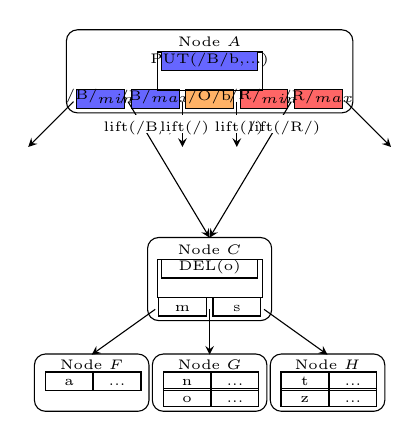
\begin{tikzpicture}[xscale=0.95, yscale=0.95]
            \node[anchor=south, rectangle, rounded corners, minimum height=.06\textwidth, minimum width=.12\textwidth, draw=black] at (-.1625\textwidth, -.1\textwidth) {};
            \node[anchor=south, font=\tiny] at (-.1625\textwidth, -.064\textwidth) {Node $F$};
            \node[anchor=south, rectangle, minimum height=.015\textwidth, minimum width=.05\textwidth, draw=black] at (-.1875\textwidth, -.077\textwidth) {};
            \node[anchor=south, font=\tiny] at (-.1875\textwidth, -.082\textwidth) {a};
            \node[anchor=south, rectangle, minimum height=.015\textwidth, minimum width=.05\textwidth, draw=black] at (-.1345\textwidth, -.077\textwidth) {};
            \node[anchor=south, font=\tiny] at (-.1345\textwidth, -.082\textwidth) {...};

            \node[anchor=south, rectangle, rounded corners, minimum height=.06\textwidth, minimum width=.12\textwidth, draw=black] at (-.0325\textwidth, -.1\textwidth) {};
            \node[anchor=south, font=\tiny] at (-.0325\textwidth, -.064\textwidth) {Node $G$};
            \node[anchor=south, rectangle, minimum height=.015\textwidth, minimum width=.05\textwidth, draw=black] at (-.0575\textwidth, -.095\textwidth) {};
            \node[anchor=south, font=\tiny] at (-.0575\textwidth, -.1\textwidth) {o};
            \node[anchor=south, rectangle, minimum height=.015\textwidth, minimum width=.05\textwidth, draw=black] at (-.0045\textwidth, -.095\textwidth) {};
            \node[anchor=south, font=\tiny] at (-.0045\textwidth, -.1\textwidth) {...};
            \node[anchor=south, rectangle, minimum height=.015\textwidth, minimum width=.05\textwidth, draw=black] at (-.0575\textwidth, -.077\textwidth) {};
            \node[anchor=south, font=\tiny] at (-.0575\textwidth, -.082\textwidth) {n};
            \node[anchor=south, rectangle, minimum height=.015\textwidth, minimum width=.05\textwidth, draw=black] at (-.0045\textwidth, -.077\textwidth) {};
            \node[anchor=south, font=\tiny] at (-.0045\textwidth, -.082\textwidth) {...};

            \node[anchor=south, rectangle, rounded corners, minimum height=.06\textwidth, minimum width=.12\textwidth, draw=black] at (.0975\textwidth, -.1\textwidth) {};
            \node[anchor=south, font=\tiny] at (.0975\textwidth, -.064\textwidth) {Node $H$};
            \node[anchor=south, rectangle, minimum height=.015\textwidth, minimum width=.05\textwidth, draw=black] at (.0725\textwidth, -.095\textwidth) {};
            \node[anchor=south, font=\tiny] at (.0725\textwidth, -.1\textwidth) {z};
            \node[anchor=south, rectangle, minimum height=.015\textwidth, minimum width=.05\textwidth, draw=black] at (.1255\textwidth, -.095\textwidth) {};
            \node[anchor=south, font=\tiny] at (.1255\textwidth, -.1\textwidth) {...};
            \node[anchor=south, rectangle, minimum height=.015\textwidth, minimum width=.05\textwidth, draw=black] at (.0725\textwidth, -.077\textwidth) {};
            \node[anchor=south, font=\tiny] at (.0725\textwidth, -.082\textwidth) {t};
            \node[anchor=south, rectangle, minimum height=.015\textwidth, minimum width=.05\textwidth, draw=black] at (.1255\textwidth, -.077\textwidth) {};
            \node[anchor=south, font=\tiny] at (.1255\textwidth, -.082\textwidth) {...};

            \node[anchor=south, rectangle, rounded corners, minimum height=.087\textwidth, minimum width=.13\textwidth, draw=black] at (-.0325\textwidth, 0) {};
            \node[anchor=south, font=\tiny] at (-.0325\textwidth, .063\textwidth) {Node $C$};
            \node[anchor=south, rectangle, minimum height=.015\textwidth, minimum width=.05\textwidth, draw=black] at (-.0625\textwidth, .005\textwidth) {};
            \node[anchor=south, font=\tiny] at (-.0625\textwidth, 0) {m};
            \node[anchor=south, rectangle, minimum height=.015\textwidth, minimum width=.05\textwidth, draw=black] at (-.0025\textwidth, .005\textwidth) {};
            \node[anchor=south, font=\tiny] at (-.0025\textwidth, 0) {s};
            \node[anchor=south, rectangle, minimum height=.04\textwidth, minimum width=.11\textwidth, draw=black] at (-.0325\textwidth, .025\textwidth) {};
            \node[anchor=south, rectangle, minimum height=.015\textwidth, minimum width=.1\textwidth, draw=black] at (-.0325\textwidth, .047\textwidth) {};
            \node[anchor=south, font=\tiny] at  (-.0325\textwidth, .041\textwidth) {DEL(o)};

            \node[anchor=south, rectangle, rounded corners, minimum height=.087\textwidth, minimum width=.3\textwidth, draw=black] at (-.0325\textwidth, .229\textwidth) {};
            \node[anchor=south, font=\tiny] at (-.0325\textwidth, .292\textwidth) {Node $A$};
            \node[anchor=south, rectangle, minimum height=.015\textwidth, minimum width=.05\textwidth, draw=black, fill={blue!60}] at (-.1525\textwidth, .234\textwidth) {};
            \node[anchor=south, font=\tiny] at (-.1525\textwidth, .229\textwidth) {/B/$_{min}$};
            \node[anchor=south, rectangle, minimum height=.015\textwidth, minimum width=.05\textwidth, draw=black, fill={blue!60}] at (-.0925\textwidth, .234\textwidth) {};
            \node[anchor=south, font=\tiny] at (-.0925\textwidth, .229\textwidth) {/B/$_{max}$};
            \node[anchor=south, rectangle, minimum height=.015\textwidth, minimum width=.05\textwidth, draw=black, fill={orange!60}] at (-.0325\textwidth, .234\textwidth) {};
            \node[anchor=south, font=\tiny] at (-.0325\textwidth, .229\textwidth) {/O/b};
            \node[anchor=south, rectangle, minimum height=.015\textwidth, minimum width=.05\textwidth, draw=black, fill={red!60}] at (.0275\textwidth, .234\textwidth) {};
            \node[anchor=south, font=\tiny] at (.0275\textwidth, .229\textwidth) {/R/$_{min}$};
            \node[anchor=south, rectangle, minimum height=.015\textwidth, minimum width=.05\textwidth, draw=black, fill={red!60}] at (.0875\textwidth, .234\textwidth) {};
            \node[anchor=south, font=\tiny] at (.0875\textwidth, .229\textwidth) {/R/$_{max}$};
            \node[anchor=south, rectangle, minimum height=.04\textwidth, minimum width=.11\textwidth, draw=black] at (-.0325\textwidth, .254\textwidth) {};
            \node[anchor=south, rectangle, minimum height=.015\textwidth, minimum width=.1\textwidth, draw=black, fill={blue!60}] at (-.0325\textwidth, .276\textwidth) {};
            \node[anchor=south, font=\tiny] at  (-.0325\textwidth, .27\textwidth) {PUT(/B/b,...)};

            \draw[->, >=stealth] (-.0325\textwidth, .013\textwidth) -- (-.0325\textwidth, -.037\textwidth);
            \draw[->, >=stealth] (.0275\textwidth, .013\textwidth) -- (.0975\textwidth, -.037\textwidth);
            \draw[->, >=stealth] (-.0925\textwidth, .013\textwidth) -- (-.1625\textwidth, -.037\textwidth);
            \draw[->, >=stealth] (-.1825\textwidth, .242\textwidth) -- (-.2325\textwidth, .192\textwidth);
            \draw[->, >=stealth] (-.1225\textwidth, .242\textwidth) -- (-.0325\textwidth, .092\textwidth);
            \draw[->, >=stealth] (-.0625\textwidth, .242\textwidth) -- (-.0625\textwidth, .192\textwidth);
            \draw[->, >=stealth] (-.0025\textwidth, .242\textwidth) -- (-.0025\textwidth, .192\textwidth);
            \draw[->, >=stealth] (.0575\textwidth, .242\textwidth) -- (-.0325\textwidth, .092\textwidth);
            \draw[->, >=stealth] (.1175\textwidth, .242\textwidth) -- (.1675\textwidth, .192\textwidth);

            \node[anchor=north,rectangle, minimum height=.015\textwidth, minimum width=.05\textwidth, fill={white}] at (-.11\textwidth, .228\textwidth) {};
            \node[anchor=north, font=\tiny] at (-.11\textwidth, .231\textwidth) {lift(/B/)};
            \node[anchor=north,rectangle, minimum height=.015\textwidth, minimum width=.05\textwidth, fill={white}] at (-.06\textwidth, .228\textwidth) {};
            \node[anchor=north, font=\tiny] at (-.06\textwidth, .231\textwidth) {lift(/)};
            \node[anchor=north,rectangle, minimum height=.015\textwidth, minimum width=.05\textwidth, fill={white}] at (0, .228\textwidth) {};
            \node[anchor=north, font=\tiny] at (0, .231\textwidth) {lift(/)};
            \node[anchor=north,rectangle, minimum height=.015\textwidth, minimum width=.05\textwidth, fill={white}] at (.05\textwidth, .228\textwidth) {};
            \node[anchor=north, font=\tiny] at (.05\textwidth, .231\textwidth) {lift(/R/)};
        \end{tikzpicture}
        \caption{\label{subfig:cow-1} Node $C'$ is a shared by two
            parent-to-child pointers in Node $A$.}
    \end{subfigure}
    \begin{subfigure}{\textwidth}
        \centering
        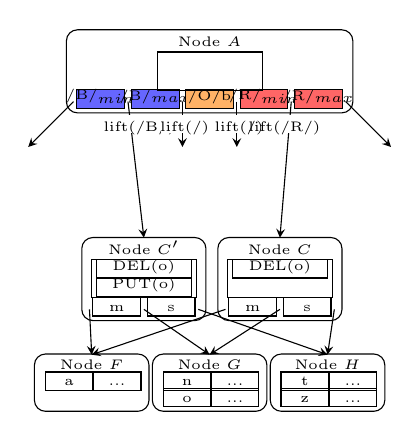
\begin{tikzpicture}[xscale=0.95, yscale=0.95]
            \node[anchor=south, rectangle, rounded corners, minimum height=.06\textwidth, minimum width=.12\textwidth, draw=black] at (-.1625\textwidth, -.1\textwidth) {};
            \node[anchor=south, font=\tiny] at (-.1625\textwidth, -.064\textwidth) {Node $F$};
            \node[anchor=south, rectangle, minimum height=.015\textwidth, minimum width=.05\textwidth, draw=black] at (-.1875\textwidth, -.077\textwidth) {};
            \node[anchor=south, font=\tiny] at (-.1875\textwidth, -.082\textwidth) {a};
            \node[anchor=south, rectangle, minimum height=.015\textwidth, minimum width=.05\textwidth, draw=black] at (-.1345\textwidth, -.077\textwidth) {};
            \node[anchor=south, font=\tiny] at (-.1345\textwidth, -.082\textwidth) {...};

            \node[anchor=south, rectangle, rounded corners, minimum height=.06\textwidth, minimum width=.12\textwidth, draw=black] at (-.0325\textwidth, -.1\textwidth) {};
            \node[anchor=south, font=\tiny] at (-.0325\textwidth, -.064\textwidth) {Node $G$};
            \node[anchor=south, rectangle, minimum height=.015\textwidth, minimum width=.05\textwidth, draw=black] at (-.0575\textwidth, -.095\textwidth) {};
            \node[anchor=south, font=\tiny] at (-.0575\textwidth, -.1\textwidth) {o};
            \node[anchor=south, rectangle, minimum height=.015\textwidth, minimum width=.05\textwidth, draw=black] at (-.0045\textwidth, -.095\textwidth) {};
            \node[anchor=south, font=\tiny] at (-.0045\textwidth, -.1\textwidth) {...};
            \node[anchor=south, rectangle, minimum height=.015\textwidth, minimum width=.05\textwidth, draw=black] at (-.0575\textwidth, -.077\textwidth) {};
            \node[anchor=south, font=\tiny] at (-.0575\textwidth, -.082\textwidth) {n};
            \node[anchor=south, rectangle, minimum height=.015\textwidth, minimum width=.05\textwidth, draw=black] at (-.0045\textwidth, -.077\textwidth) {};
            \node[anchor=south, font=\tiny] at (-.0045\textwidth, -.082\textwidth) {...};

            \node[anchor=south, rectangle, rounded corners, minimum height=.06\textwidth, minimum width=.12\textwidth, draw=black] at (.0975\textwidth, -.1\textwidth) {};
            \node[anchor=south, font=\tiny] at (.0975\textwidth, -.064\textwidth) {Node $H$};
            \node[anchor=south, rectangle, minimum height=.015\textwidth, minimum width=.05\textwidth, draw=black] at (.0725\textwidth, -.095\textwidth) {};
            \node[anchor=south, font=\tiny] at (.0725\textwidth, -.1\textwidth) {z};
            \node[anchor=south, rectangle, minimum height=.015\textwidth, minimum width=.05\textwidth, draw=black] at (.1255\textwidth, -.095\textwidth) {};
            \node[anchor=south, font=\tiny] at (.1255\textwidth, -.1\textwidth) {...};
            \node[anchor=south, rectangle, minimum height=.015\textwidth, minimum width=.05\textwidth, draw=black] at (.0725\textwidth, -.077\textwidth) {};
            \node[anchor=south, font=\tiny] at (.0725\textwidth, -.082\textwidth) {t};
            \node[anchor=south, rectangle, minimum height=.015\textwidth, minimum width=.05\textwidth, draw=black] at (.1255\textwidth, -.077\textwidth) {};
            \node[anchor=south, font=\tiny] at (.1255\textwidth, -.082\textwidth) {...};

            \node[anchor=south, rectangle, rounded corners, minimum height=.087\textwidth, minimum width=.13\textwidth, draw=black] at (.045\textwidth, 0) {};
            \node[anchor=south, font=\tiny] at (.045\textwidth, .063\textwidth) {Node $C$};
            \node[anchor=south, rectangle, minimum height=.015\textwidth, minimum width=.05\textwidth, draw=black] at (.015\textwidth, .005\textwidth) {};
            \node[anchor=south, font=\tiny] at (.015\textwidth, 0) {m};
            \node[anchor=south, rectangle, minimum height=.015\textwidth, minimum width=.05\textwidth, draw=black] at (.075\textwidth, .005\textwidth) {};
            \node[anchor=south, font=\tiny] at (.075\textwidth, 0) {s};
            \node[anchor=south, rectangle, minimum height=.04\textwidth, minimum width=.11\textwidth, draw=black] at (.045\textwidth, .025\textwidth) {};
            \node[anchor=south, rectangle, minimum height=.015\textwidth, minimum width=.1\textwidth, draw=black] at (.045\textwidth, .047\textwidth) {};
            \node[anchor=south, font=\tiny] at  (.045\textwidth, .041\textwidth) {DEL(o)};

            \node[anchor=south, rectangle, rounded corners, minimum height=.087\textwidth, minimum width=.13\textwidth, draw=black] at (-.105\textwidth, 0) {};
            \node[anchor=south, font=\tiny] at (-.105\textwidth, .063\textwidth) {Node $C'$};
            \node[anchor=south, rectangle, minimum height=.015\textwidth, minimum width=.05\textwidth, draw=black] at (-.135\textwidth, .005\textwidth) {};
            \node[anchor=south, font=\tiny] at (-.135\textwidth, 0) {m};
            \node[anchor=south, rectangle, minimum height=.015\textwidth, minimum width=.05\textwidth, draw=black] at (-.075\textwidth, .005\textwidth) {};
            \node[anchor=south, font=\tiny] at (-.075\textwidth, 0) {s};
            \node[anchor=south, rectangle, minimum height=.04\textwidth, minimum width=.11\textwidth, draw=black] at (-.105\textwidth, .025\textwidth) {};
            \node[anchor=south, rectangle, minimum height=.015\textwidth, minimum width=.1\textwidth, draw=black] at (-.105\textwidth, .047\textwidth) {};
            \node[anchor=south, font=\tiny] at  (-.105\textwidth, .041\textwidth) {DEL(o)};
            \node[anchor=south, rectangle, minimum height=.015\textwidth, minimum width=.1\textwidth, draw=black] at (-.105\textwidth, .027\textwidth) {};
            \node[anchor=south, font=\tiny] at  (-.105\textwidth, .021\textwidth) {PUT(o)};

            \node[anchor=south, rectangle, rounded corners, minimum height=.087\textwidth, minimum width=.3\textwidth, draw=black] at (-.0325\textwidth, .229\textwidth) {};
            \node[anchor=south, font=\tiny] at (-.0325\textwidth, .292\textwidth) {Node $A$};
            \node[anchor=south, rectangle, minimum height=.015\textwidth, minimum width=.05\textwidth, draw=black, fill={blue!60}] at (-.1525\textwidth, .234\textwidth) {};
            \node[anchor=south, font=\tiny] at (-.1525\textwidth, .229\textwidth) {/B/$_{min}$};
            \node[anchor=south, rectangle, minimum height=.015\textwidth, minimum width=.05\textwidth, draw=black, fill={blue!60}] at (-.0925\textwidth, .234\textwidth) {};
            \node[anchor=south, font=\tiny] at (-.0925\textwidth, .229\textwidth) {/B/$_{max}$};
            \node[anchor=south, rectangle, minimum height=.015\textwidth, minimum width=.05\textwidth, draw=black, fill={orange!60}] at (-.0325\textwidth, .234\textwidth) {};
            \node[anchor=south, font=\tiny] at (-.0325\textwidth, .229\textwidth) {/O/b};
            \node[anchor=south, rectangle, minimum height=.015\textwidth, minimum width=.05\textwidth, draw=black, fill={red!60}] at (.0275\textwidth, .234\textwidth) {};
            \node[anchor=south, font=\tiny] at (.0275\textwidth, .229\textwidth) {/R/$_{min}$};
            \node[anchor=south, rectangle, minimum height=.015\textwidth, minimum width=.05\textwidth, draw=black, fill={red!60}] at (.0875\textwidth, .234\textwidth) {};
            \node[anchor=south, font=\tiny] at (.0875\textwidth, .229\textwidth) {/R/$_{max}$};
            \node[anchor=south, rectangle, minimum height=.04\textwidth, minimum width=.11\textwidth, draw=black] at (-.0325\textwidth, .254\textwidth) {};

            \draw[->, >=stealth] (-.105\textwidth, .013\textwidth) -- (-.0325\textwidth, -.037\textwidth);
            \draw[->, >=stealth] (-.045\textwidth, .013\textwidth) -- (.0975\textwidth, -.037\textwidth);
            \draw[->, >=stealth] (-.165\textwidth, .013\textwidth) -- (-.1625\textwidth, -.037\textwidth);
            \draw[->, >=stealth] (.045\textwidth, .013\textwidth) -- (-.0325\textwidth, -.037\textwidth);
            \draw[->, >=stealth] (.105\textwidth, .013\textwidth) -- (.0975\textwidth, -.037\textwidth);
            \draw[->, >=stealth] (-.015\textwidth, .013\textwidth) -- (-.1625\textwidth, -.037\textwidth);
            \draw[->, >=stealth] (-.1825\textwidth, .242\textwidth) -- (-.2325\textwidth, .192\textwidth);
            \draw[->, >=stealth] (-.1225\textwidth, .242\textwidth) -- (-.105\textwidth, .092\textwidth);
            \draw[->, >=stealth] (-.0625\textwidth, .242\textwidth) -- (-.0625\textwidth, .192\textwidth);
            \draw[->, >=stealth] (-.0025\textwidth, .242\textwidth) -- (-.0025\textwidth, .192\textwidth);
            \draw[->, >=stealth] (.0575\textwidth, .242\textwidth) -- (.045\textwidth, .092\textwidth);
            \draw[->, >=stealth] (.1175\textwidth, .242\textwidth) -- (.1675\textwidth, .192\textwidth);

            \node[anchor=north,rectangle, minimum height=.015\textwidth, minimum width=.05\textwidth, fill={white}] at (-.11\textwidth, .228\textwidth) {};
            \node[anchor=north, font=\tiny] at (-.11\textwidth, .231\textwidth) {lift(/B/)};
            \node[anchor=north,rectangle, minimum height=.015\textwidth, minimum width=.05\textwidth, fill={white}] at (-.06\textwidth, .228\textwidth) {};
            \node[anchor=north, font=\tiny] at (-.06\textwidth, .231\textwidth) {lift(/)};
            \node[anchor=north,rectangle, minimum height=.015\textwidth, minimum width=.05\textwidth, fill={white}] at (0, .228\textwidth) {};
            \node[anchor=north, font=\tiny] at (0, .231\textwidth) {lift(/)};
            \node[anchor=north,rectangle, minimum height=.015\textwidth, minimum width=.05\textwidth, fill={white}] at (.05\textwidth, .228\textwidth) {};
            \node[anchor=north, font=\tiny] at (.05\textwidth, .231\textwidth) {lift(/R/)};
        \end{tikzpicture}
        \caption{\label{subfig:cow-2} Before Node $A$ flushes ``/B/'' messages,
            it breaks the sharing creating Node $C''$, which is a clone of Node
            $C'$.}
    \end{subfigure}
    \caption[\bedags break node sharing with CoW]{\label{fig:cow}
        When the parent accumulates enough messages to flush to a shared node,
        it breaks the sharing with Cow.}
\end{figure}

Any writes to a shared node must first break the sharing of the node, the
\bedag maintains reference counting for each node to track the sharing status of
nodes.
In particular, \fti has a node table that maps node IDs to physical locations on
disk.
The \bedag stores the reference count of each node in the node table alongside
the mapping.
Before writing to a node, the \bedag must check the reference count of the node.

The \bedag breaks the sharing of a node using Copy-on-Write (CoW).
After range-rename, one parent of the shared node might choose to flush its
messages to the node.
At this moment, the lifted \bedag creates a new node that is identical to the
shared node, sharing all children of the node.
The lifted \bedag then sets the parent-to-child pointer to the new node and
performs the flush.

Figure~\ref{fig:cow} shows an example of the CoW process.
In Figure~\ref{subfig:cow-1}, Node $A$ has two parent-to-child pointers to
Node $C'$ with reference count 2.
Note, Node $F'$, $G$ and $H'$ have reference count 1.
When Node $A$ accumulates enough messages and wants to flush messages with
``/B/'', it clones Node $C'$ to break the sharing.
As shown in Figure~\ref{subfig:cow-2}, the \bedag creates a new Node $C''$
identical to Node $C'$.
Now, both Node $C'$ and $C''$ have reference count, while Node $F'$, $G$ and
$H'$ have reference count 2.

\subsection{\goto messages}

Instead of performing all works on the critical path, range-clone can use a
new type of messages, the \goto message, that delays tree surgery to flushes
in the lifted \bedag.

A \goto message consists of 3 parts: a \dpre, a \spre, a node ID.
When a query visits a node during its root-to-leaf traversal, it must check
\goto messages.
If the \dpre of a \goto message matches the search key, the query should follow
the \goto message, instead of the parent-to-child pointer in the node.
In other words, the next node this query visit should be the node whose node ID
is in the \goto message.
Also, the query should update its search key by changing the prefix from \dpre
to \spre.
If the query finds multiple \goto messages matching its search key, it follows
the \goto message with the latest timestamp.

A \goto message serves two purposes:
\begin{itemize}
\item it works as additional parent-to-child pointers in the node.
Additionally, it works as a filter.
For all keys the query gets following the \goto messages, only keys with \spre
are valid.
\item it nullifies messages that have the destination key and an older
timestamp, because those messages cannot stay higher than the \goto message.
\end{itemize}
\goto messages can be used to implement range-query messages by setting the node
ID to a special value (e.g., 0).

\begin{figure}
    \begin{subfigure}{\textwidth}
        \centering
        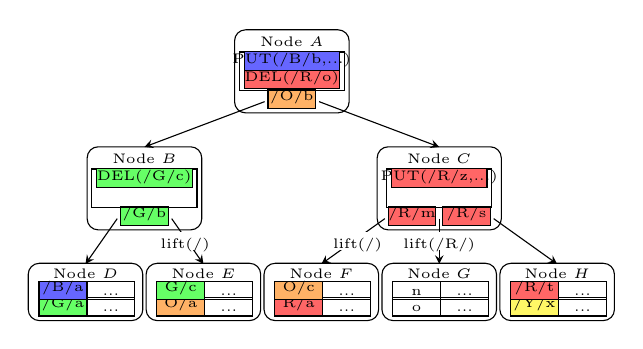
\begin{tikzpicture}[xscale=0.95, yscale=0.95]
            \node[anchor=south, rectangle, rounded corners, minimum height=.06\textwidth, minimum width=.12\textwidth, draw=black] at (0, 0) {};
            \node[anchor=south, font=\tiny] at (0, .036\textwidth) {Node $F$};
            \node[anchor=south, rectangle, minimum height=.015\textwidth, minimum width=.05\textwidth, draw=black, fill={red!60}] at (-.025\textwidth, .005\textwidth) {};
            \node[anchor=south, font=\tiny] at (-.025\textwidth, 0) {R/a};
            \node[anchor=south, rectangle, minimum height=.015\textwidth, minimum width=.05\textwidth, draw=black] at (.028\textwidth, .005\textwidth) {};
            \node[anchor=south, font=\tiny] at (.028\textwidth, 0) {...};
            \node[anchor=south, rectangle, minimum height=.015\textwidth, minimum width=.05\textwidth, draw=black, fill={orange!60}] at (-.025\textwidth, .023\textwidth) {};
            \node[anchor=south, font=\tiny] at (-.025\textwidth, .018\textwidth) {O/c};
            \node[anchor=south, rectangle, minimum height=.015\textwidth, minimum width=.05\textwidth, draw=black] at (.028\textwidth, .023\textwidth) {};
            \node[anchor=south, font=\tiny] at (.028\textwidth, .018\textwidth) {...};

            \node[anchor=south, rectangle, rounded corners, minimum height=.06\textwidth, minimum width=.12\textwidth, draw=black] at (.13\textwidth, 0) {};
            \node[anchor=south, font=\tiny] at (.13\textwidth, .036\textwidth) {Node $G$};
            \node[anchor=south, rectangle, minimum height=.015\textwidth, minimum width=.05\textwidth, draw=black] at (.105\textwidth, .005\textwidth) {};
            \node[anchor=south, font=\tiny] at (.105\textwidth, 0) {o};
            \node[anchor=south, rectangle, minimum height=.015\textwidth, minimum width=.05\textwidth, draw=black] at (.158\textwidth, .005\textwidth) {};
            \node[anchor=south, font=\tiny] at (.158\textwidth, 0) {...};
            \node[anchor=south, rectangle, minimum height=.015\textwidth, minimum width=.05\textwidth, draw=black] at (.105\textwidth, .023\textwidth) {};
            \node[anchor=south, font=\tiny] at (.105\textwidth, .018\textwidth) {n};
            \node[anchor=south, rectangle, minimum height=.015\textwidth, minimum width=.05\textwidth, draw=black] at (.158\textwidth, .023\textwidth) {};
            \node[anchor=south, font=\tiny] at (.158\textwidth, .018\textwidth) {...};

            \node[anchor=south, rectangle, rounded corners, minimum height=.06\textwidth, minimum width=.12\textwidth, draw=black] at (.26\textwidth, 0) {};
            \node[anchor=south, font=\tiny] at (.26\textwidth, .036\textwidth) {Node $H$};
            \node[anchor=south, rectangle, minimum height=.015\textwidth, minimum width=.05\textwidth, draw=black, fill={yellow!60}] at (.235\textwidth, .005\textwidth) {};
            \node[anchor=south, font=\tiny] at (.235\textwidth, 0) {/Y/x};
            \node[anchor=south, rectangle, minimum height=.015\textwidth, minimum width=.05\textwidth, draw=black] at (.288\textwidth, .005\textwidth) {};
            \node[anchor=south, font=\tiny] at (.288\textwidth, 0) {...};
            \node[anchor=south, rectangle, minimum height=.015\textwidth, minimum width=.05\textwidth, draw=black, fill={red!60}] at (.235\textwidth, .023\textwidth) {};
            \node[anchor=south, font=\tiny] at (.235\textwidth, .018\textwidth) {/R/t};
            \node[anchor=south, rectangle, minimum height=.015\textwidth, minimum width=.05\textwidth, draw=black] at (.288\textwidth, .023\textwidth) {};
            \node[anchor=south, font=\tiny] at (.288\textwidth, .018\textwidth) {...};

            \node[anchor=south, rectangle, rounded corners, minimum height=.06\textwidth, minimum width=.12\textwidth, draw=black] at (-.13\textwidth, 0) {};
            \node[anchor=south, font=\tiny] at (-.13\textwidth, .036\textwidth) {Node $E$};
            \node[anchor=south, rectangle, minimum height=.015\textwidth, minimum width=.05\textwidth, draw=black, fill={orange!60}] at (-.155\textwidth, .005\textwidth) {};
            \node[anchor=south, font=\tiny] at (-.155\textwidth, 0) {O/a};
            \node[anchor=south, rectangle, minimum height=.015\textwidth, minimum width=.05\textwidth, draw=black] at (-.102\textwidth, .005\textwidth) {};
            \node[anchor=south, font=\tiny] at (-.102\textwidth, 0) {...};
            \node[anchor=south, rectangle, minimum height=.015\textwidth, minimum width=.05\textwidth, draw=black, fill={green!60}] at (-.155\textwidth, .023\textwidth) {};
            \node[anchor=south, font=\tiny] at (-.155\textwidth, .018\textwidth) {G/c};
            \node[anchor=south, rectangle, minimum height=.015\textwidth, minimum width=.05\textwidth, draw=black] at (-.102\textwidth, .023\textwidth) {};
            \node[anchor=south, font=\tiny] at (-.102\textwidth, .018\textwidth) {...};

            \node[anchor=south, rectangle, rounded corners, minimum height=.06\textwidth, minimum width=.12\textwidth, draw=black] at (-.26\textwidth, 0) {};
            \node[anchor=south, font=\tiny] at (-.26\textwidth, .036\textwidth) {Node $D$};
            \node[anchor=south, rectangle, minimum height=.015\textwidth, minimum width=.05\textwidth, draw=black, fill={green!60}] at (-.285\textwidth, .005\textwidth) {};
            \node[anchor=south, font=\tiny] at (-.285\textwidth, 0) {/G/a};
            \node[anchor=south, rectangle, minimum height=.015\textwidth, minimum width=.05\textwidth, draw=black] at (-.232\textwidth, .005\textwidth) {};
            \node[anchor=south, font=\tiny] at (-.232\textwidth, 0) {...};
            \node[anchor=south, rectangle, minimum height=.015\textwidth, minimum width=.05\textwidth, draw=black, fill={blue!60}] at (-.285\textwidth, .023\textwidth) {};
            \node[anchor=south, font=\tiny] at (-.285\textwidth, .018\textwidth) {/B/a};
            \node[anchor=south, rectangle, minimum height=.015\textwidth, minimum width=.05\textwidth, draw=black] at (-.232\textwidth, .023\textwidth) {};
            \node[anchor=south, font=\tiny] at (-.232\textwidth, .018\textwidth) {...};

            \node[anchor=south, rectangle, rounded corners, minimum height=.087\textwidth, minimum width=.12\textwidth, draw=black] at (-.195\textwidth, .1\textwidth) {};
            \node[anchor=south, font=\tiny] at (-.195\textwidth, .163\textwidth) {Node $B$};
            \node[anchor=south, rectangle, minimum height=.015\textwidth, minimum width=.05\textwidth, draw=black, fill={green!60}] at (-.195\textwidth, .105\textwidth) {};
            \node[anchor=south, font=\tiny] at (-.195\textwidth, .1\textwidth) {/G/b};
            \node[anchor=south, rectangle, minimum height=.04\textwidth, minimum width=.11\textwidth, draw=black] at (-.195\textwidth, .125\textwidth) {};
            \node[anchor=south, rectangle, minimum height=.015\textwidth, minimum width=.1\textwidth, draw=black, fill={green!60}] at (-.195\textwidth, .147\textwidth) {};
            \node[anchor=south, font=\tiny] at  (-.195\textwidth, .141\textwidth) {DEL(/G/c)};

            \node[anchor=south, rectangle, rounded corners, minimum height=.087\textwidth, minimum width=.13\textwidth, draw=black] at (.13\textwidth, .1\textwidth) {};
            \node[anchor=south, font=\tiny] at (.13\textwidth, .163\textwidth) {Node $C$};
            \node[anchor=south, rectangle, minimum height=.015\textwidth, minimum width=.05\textwidth, draw=black, fill={red!60}] at (.1\textwidth, .105\textwidth) {};
            \node[anchor=south, font=\tiny] at (.1\textwidth, .1\textwidth) {/R/m};
            \node[anchor=south, rectangle, minimum height=.015\textwidth, minimum width=.05\textwidth, draw=black, fill={red!60}] at (.16\textwidth, .105\textwidth) {};
            \node[anchor=south, font=\tiny] at (.16\textwidth, .1\textwidth) {/R/s};
            \node[anchor=south, rectangle, minimum height=.04\textwidth, minimum width=.11\textwidth, draw=black] at (.13\textwidth, .125\textwidth) {};
            \node[anchor=south, rectangle, minimum height=.015\textwidth, minimum width=.1\textwidth, draw=black, fill={red!60}] at (.13\textwidth, .147\textwidth) {};
            \node[anchor=south, font=\tiny] at  (.13\textwidth, .141\textwidth) {PUT(/R/z,...)};

            \node[anchor=south, rectangle, rounded corners, minimum height=.087\textwidth, minimum width=.12\textwidth, draw=black] at (-.0325\textwidth, .229\textwidth) {};
            \node[anchor=south, font=\tiny] at (-.0325\textwidth, .292\textwidth) {Node $A$};
            \node[anchor=south, rectangle, minimum height=.015\textwidth, minimum width=.05\textwidth, draw=black, fill={orange!60}] at (-.0325\textwidth, .234\textwidth) {};
            \node[anchor=south, font=\tiny] at (-.0325\textwidth, .229\textwidth) {/O/b};
            \node[anchor=south, rectangle, minimum height=.04\textwidth, minimum width=.11\textwidth, draw=black] at (-.0325\textwidth, .254\textwidth) {};
            \node[anchor=south, rectangle, minimum height=.015\textwidth, minimum width=.1\textwidth, draw=black, fill={red!60}] at (-.0325\textwidth, .256\textwidth) {};
            \node[anchor=south, font=\tiny] at  (-.0325\textwidth, .25\textwidth) {DEL(/R/o)};
            \node[anchor=south, rectangle, minimum height=.015\textwidth, minimum width=.1\textwidth, draw=black, fill={blue!60}] at (-.0325\textwidth, .276\textwidth) {};
            \node[anchor=south, font=\tiny] at  (-.0325\textwidth, .27\textwidth) {PUT(/B/b,...)};

            \draw[->, >=stealth] (-.225\textwidth, .113\textwidth) -- (-.26\textwidth, .063\textwidth);
            \draw[->, >=stealth] (-.165\textwidth, .113\textwidth) -- (-.13\textwidth, .063\textwidth);
            \draw[->, >=stealth] (.13\textwidth, .113\textwidth) -- (.13\textwidth, .063\textwidth);
            \draw[->, >=stealth] (.19\textwidth, .113\textwidth) -- (.26\textwidth, .063\textwidth);
            \draw[->, >=stealth] (.07\textwidth, .113\textwidth) -- (0, .063\textwidth);
            \draw[->, >=stealth] (-.0625\textwidth, .242\textwidth) -- (-.195\textwidth, .192\textwidth);
            \draw[->, >=stealth] (-.0025\textwidth, .242\textwidth) -- (.13\textwidth, .192\textwidth);

            \node[anchor=north,rectangle, minimum height=.015\textwidth, minimum width=.05\textwidth, fill={white}] at (.13\textwidth, .099\textwidth) {};
            \node[anchor=north, font=\tiny] at (.13\textwidth, .102\textwidth) {lift(/R/)};
            \node[anchor=north,rectangle, minimum height=.015\textwidth, minimum width=.05\textwidth, fill={white}] at (.04\textwidth, .099\textwidth) {};
            \node[anchor=north, font=\tiny] at (.04\textwidth, .102\textwidth) {lift(/)};
            \node[anchor=north,rectangle, minimum height=.015\textwidth, minimum width=.05\textwidth, fill={white}] at (-.15\textwidth, .099\textwidth) {};
            \node[anchor=north, font=\tiny] at (-.15\textwidth, .102\textwidth) {lift(/)};
        \end{tikzpicture}
        \caption{\label{subfig:goto-1} The \bet before the range-clone.}
    \end{subfigure}
    \begin{subfigure}{\textwidth}
        \centering
        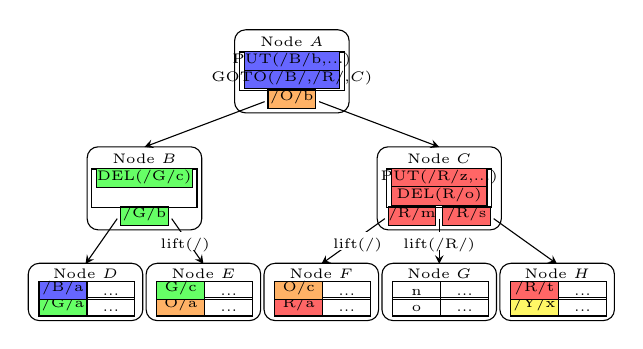
\begin{tikzpicture}[xscale=0.95, yscale=0.95]
            \node[anchor=south, rectangle, rounded corners, minimum height=.06\textwidth, minimum width=.12\textwidth, draw=black] at (0, 0) {};
            \node[anchor=south, font=\tiny] at (0, .036\textwidth) {Node $F$};
            \node[anchor=south, rectangle, minimum height=.015\textwidth, minimum width=.05\textwidth, draw=black, fill={red!60}] at (-.025\textwidth, .005\textwidth) {};
            \node[anchor=south, font=\tiny] at (-.025\textwidth, 0) {R/a};
            \node[anchor=south, rectangle, minimum height=.015\textwidth, minimum width=.05\textwidth, draw=black] at (.028\textwidth, .005\textwidth) {};
            \node[anchor=south, font=\tiny] at (.028\textwidth, 0) {...};
            \node[anchor=south, rectangle, minimum height=.015\textwidth, minimum width=.05\textwidth, draw=black, fill={orange!60}] at (-.025\textwidth, .023\textwidth) {};
            \node[anchor=south, font=\tiny] at (-.025\textwidth, .018\textwidth) {O/c};
            \node[anchor=south, rectangle, minimum height=.015\textwidth, minimum width=.05\textwidth, draw=black] at (.028\textwidth, .023\textwidth) {};
            \node[anchor=south, font=\tiny] at (.028\textwidth, .018\textwidth) {...};

            \node[anchor=south, rectangle, rounded corners, minimum height=.06\textwidth, minimum width=.12\textwidth, draw=black] at (.13\textwidth, 0) {};
            \node[anchor=south, font=\tiny] at (.13\textwidth, .036\textwidth) {Node $G$};
            \node[anchor=south, rectangle, minimum height=.015\textwidth, minimum width=.05\textwidth, draw=black] at (.105\textwidth, .005\textwidth) {};
            \node[anchor=south, font=\tiny] at (.105\textwidth, 0) {o};
            \node[anchor=south, rectangle, minimum height=.015\textwidth, minimum width=.05\textwidth, draw=black] at (.158\textwidth, .005\textwidth) {};
            \node[anchor=south, font=\tiny] at (.158\textwidth, 0) {...};
            \node[anchor=south, rectangle, minimum height=.015\textwidth, minimum width=.05\textwidth, draw=black] at (.105\textwidth, .023\textwidth) {};
            \node[anchor=south, font=\tiny] at (.105\textwidth, .018\textwidth) {n};
            \node[anchor=south, rectangle, minimum height=.015\textwidth, minimum width=.05\textwidth, draw=black] at (.158\textwidth, .023\textwidth) {};
            \node[anchor=south, font=\tiny] at (.158\textwidth, .018\textwidth) {...};

            \node[anchor=south, rectangle, rounded corners, minimum height=.06\textwidth, minimum width=.12\textwidth, draw=black] at (.26\textwidth, 0) {};
            \node[anchor=south, font=\tiny] at (.26\textwidth, .036\textwidth) {Node $H$};
            \node[anchor=south, rectangle, minimum height=.015\textwidth, minimum width=.05\textwidth, draw=black, fill={yellow!60}] at (.235\textwidth, .005\textwidth) {};
            \node[anchor=south, font=\tiny] at (.235\textwidth, 0) {/Y/x};
            \node[anchor=south, rectangle, minimum height=.015\textwidth, minimum width=.05\textwidth, draw=black] at (.288\textwidth, .005\textwidth) {};
            \node[anchor=south, font=\tiny] at (.288\textwidth, 0) {...};
            \node[anchor=south, rectangle, minimum height=.015\textwidth, minimum width=.05\textwidth, draw=black, fill={red!60}] at (.235\textwidth, .023\textwidth) {};
            \node[anchor=south, font=\tiny] at (.235\textwidth, .018\textwidth) {/R/t};
            \node[anchor=south, rectangle, minimum height=.015\textwidth, minimum width=.05\textwidth, draw=black] at (.288\textwidth, .023\textwidth) {};
            \node[anchor=south, font=\tiny] at (.288\textwidth, .018\textwidth) {...};

            \node[anchor=south, rectangle, rounded corners, minimum height=.06\textwidth, minimum width=.12\textwidth, draw=black] at (-.13\textwidth, 0) {};
            \node[anchor=south, font=\tiny] at (-.13\textwidth, .036\textwidth) {Node $E$};
            \node[anchor=south, rectangle, minimum height=.015\textwidth, minimum width=.05\textwidth, draw=black, fill={orange!60}] at (-.155\textwidth, .005\textwidth) {};
            \node[anchor=south, font=\tiny] at (-.155\textwidth, 0) {O/a};
            \node[anchor=south, rectangle, minimum height=.015\textwidth, minimum width=.05\textwidth, draw=black] at (-.102\textwidth, .005\textwidth) {};
            \node[anchor=south, font=\tiny] at (-.102\textwidth, 0) {...};
            \node[anchor=south, rectangle, minimum height=.015\textwidth, minimum width=.05\textwidth, draw=black, fill={green!60}] at (-.155\textwidth, .023\textwidth) {};
            \node[anchor=south, font=\tiny] at (-.155\textwidth, .018\textwidth) {G/c};
            \node[anchor=south, rectangle, minimum height=.015\textwidth, minimum width=.05\textwidth, draw=black] at (-.102\textwidth, .023\textwidth) {};
            \node[anchor=south, font=\tiny] at (-.102\textwidth, .018\textwidth) {...};

            \node[anchor=south, rectangle, rounded corners, minimum height=.06\textwidth, minimum width=.12\textwidth, draw=black] at (-.26\textwidth, 0) {};
            \node[anchor=south, font=\tiny] at (-.26\textwidth, .036\textwidth) {Node $D$};
            \node[anchor=south, rectangle, minimum height=.015\textwidth, minimum width=.05\textwidth, draw=black, fill={green!60}] at (-.285\textwidth, .005\textwidth) {};
            \node[anchor=south, font=\tiny] at (-.285\textwidth, 0) {/G/a};
            \node[anchor=south, rectangle, minimum height=.015\textwidth, minimum width=.05\textwidth, draw=black] at (-.232\textwidth, .005\textwidth) {};
            \node[anchor=south, font=\tiny] at (-.232\textwidth, 0) {...};
            \node[anchor=south, rectangle, minimum height=.015\textwidth, minimum width=.05\textwidth, draw=black, fill={blue!60}] at (-.285\textwidth, .023\textwidth) {};
            \node[anchor=south, font=\tiny] at (-.285\textwidth, .018\textwidth) {/B/a};
            \node[anchor=south, rectangle, minimum height=.015\textwidth, minimum width=.05\textwidth, draw=black] at (-.232\textwidth, .023\textwidth) {};
            \node[anchor=south, font=\tiny] at (-.232\textwidth, .018\textwidth) {...};

            \node[anchor=south, rectangle, rounded corners, minimum height=.087\textwidth, minimum width=.12\textwidth, draw=black] at (-.195\textwidth, .1\textwidth) {};
            \node[anchor=south, font=\tiny] at (-.195\textwidth, .163\textwidth) {Node $B$};
            \node[anchor=south, rectangle, minimum height=.015\textwidth, minimum width=.05\textwidth, draw=black, fill={green!60}] at (-.195\textwidth, .105\textwidth) {};
            \node[anchor=south, font=\tiny] at (-.195\textwidth, .1\textwidth) {/G/b};
            \node[anchor=south, rectangle, minimum height=.04\textwidth, minimum width=.11\textwidth, draw=black] at (-.195\textwidth, .125\textwidth) {};
            \node[anchor=south, rectangle, minimum height=.015\textwidth, minimum width=.1\textwidth, draw=black, fill={green!60}] at (-.195\textwidth, .147\textwidth) {};
            \node[anchor=south, font=\tiny] at  (-.195\textwidth, .141\textwidth) {DEL(/G/c)};

            \node[anchor=south, rectangle, rounded corners, minimum height=.087\textwidth, minimum width=.13\textwidth, draw=black] at (.13\textwidth, .1\textwidth) {};
            \node[anchor=south, font=\tiny] at (.13\textwidth, .163\textwidth) {Node $C$};
            \node[anchor=south, rectangle, minimum height=.015\textwidth, minimum width=.05\textwidth, draw=black, fill={red!60}] at (.1\textwidth, .105\textwidth) {};
            \node[anchor=south, font=\tiny] at (.1\textwidth, .1\textwidth) {/R/m};
            \node[anchor=south, rectangle, minimum height=.015\textwidth, minimum width=.05\textwidth, draw=black, fill={red!60}] at (.16\textwidth, .105\textwidth) {};
            \node[anchor=south, font=\tiny] at (.16\textwidth, .1\textwidth) {/R/s};
            \node[anchor=south, rectangle, minimum height=.04\textwidth, minimum width=.11\textwidth, draw=black] at (.13\textwidth, .125\textwidth) {};
            \node[anchor=south, rectangle, minimum height=.015\textwidth, minimum width=.1\textwidth, draw=black, fill={red!60}] at (.13\textwidth, .147\textwidth) {};
            \node[anchor=south, font=\tiny] at  (.13\textwidth, .141\textwidth) {PUT(/R/z,...)};
            \node[anchor=south, rectangle, minimum height=.015\textwidth, minimum width=.1\textwidth, draw=black, fill={red!60}] at (.13\textwidth, .127\textwidth) {};
            \node[anchor=south, font=\tiny] at  (.13\textwidth, .121\textwidth) {DEL(R/o)};

            \node[anchor=south, rectangle, rounded corners, minimum height=.087\textwidth, minimum width=.12\textwidth, draw=black] at (-.0325\textwidth, .229\textwidth) {};
            \node[anchor=south, font=\tiny] at (-.0325\textwidth, .292\textwidth) {Node $A$};
            \node[anchor=south, rectangle, minimum height=.015\textwidth, minimum width=.05\textwidth, draw=black, fill={orange!60}] at (-.0325\textwidth, .234\textwidth) {};
            \node[anchor=south, font=\tiny] at (-.0325\textwidth, .229\textwidth) {/O/b};
            \node[anchor=south, rectangle, minimum height=.04\textwidth, minimum width=.11\textwidth, draw=black] at (-.0325\textwidth, .254\textwidth) {};
            \node[anchor=south, rectangle, minimum height=.015\textwidth, minimum width=.1\textwidth, draw=black, fill={blue!60}] at (-.0325\textwidth, .256\textwidth) {};
            \node[anchor=south, font=\tiny] at  (-.0325\textwidth, .25\textwidth) {GOTO(/B/,/R/,$C$)};
            \node[anchor=south, rectangle, minimum height=.015\textwidth, minimum width=.1\textwidth, draw=black, fill={blue!60}] at (-.0325\textwidth, .276\textwidth) {};
            \node[anchor=south, font=\tiny] at  (-.0325\textwidth, .27\textwidth) {PUT(/B/b,...)};

            \draw[->, >=stealth] (-.225\textwidth, .113\textwidth) -- (-.26\textwidth, .063\textwidth);
            \draw[->, >=stealth] (-.165\textwidth, .113\textwidth) -- (-.13\textwidth, .063\textwidth);
            \draw[->, >=stealth] (.13\textwidth, .113\textwidth) -- (.13\textwidth, .063\textwidth);
            \draw[->, >=stealth] (.19\textwidth, .113\textwidth) -- (.26\textwidth, .063\textwidth);
            \draw[->, >=stealth] (.07\textwidth, .113\textwidth) -- (0, .063\textwidth);
            \draw[->, >=stealth] (-.0625\textwidth, .242\textwidth) -- (-.195\textwidth, .192\textwidth);
            \draw[->, >=stealth] (-.0025\textwidth, .242\textwidth) -- (.13\textwidth, .192\textwidth);

            \node[anchor=north,rectangle, minimum height=.015\textwidth, minimum width=.05\textwidth, fill={white}] at (.13\textwidth, .099\textwidth) {};
            \node[anchor=north, font=\tiny] at (.13\textwidth, .102\textwidth) {lift(/R/)};
            \node[anchor=north,rectangle, minimum height=.015\textwidth, minimum width=.05\textwidth, fill={white}] at (.04\textwidth, .099\textwidth) {};
            \node[anchor=north, font=\tiny] at (.04\textwidth, .102\textwidth) {lift(/)};
            \node[anchor=north,rectangle, minimum height=.015\textwidth, minimum width=.05\textwidth, fill={white}] at (-.15\textwidth, .099\textwidth) {};
            \node[anchor=north, font=\tiny] at (-.15\textwidth, .102\textwidth) {lift(/)};
        \end{tikzpicture}
        \caption{\label{subfig:goto-2} The range-clone generates a \goto message
            for destination (``/B/'') keys.}
    \end{subfigure}
    \caption[A range-clone example with a \goto message]{\label{fig:goto}
        An example of range-clone(``/R/'', ``/B/'') with a \goto message.}
\end{figure}

Range-clone(\spre, \dpre) can be done with \goto messages with the following
steps:
\begin{itemize}
\item it performs a root-to-leaf traversal with \spre until reaching the source
LCA, flushing messages from parent to child simultaneously.
At this point, all messages with source keys are in the subtree rooted at the
source LCA.
\item Then it injects a \goto message into the root of the lifted \bedag with
the source LCA as the node ID in the \goto message, increasing the reference
count of the source LCA by 1.
Note, the \spre in the \goto can be different from the \spre of the range-clone,
because the root-to-leaf traversal may lift some prefix from the \spre.
\end{itemize}
Note, this range-clone design doesn't perform any tree surgery on the critical
path.

Figure~\ref{fig:goto} shows an example of range-clone(``/R/'', ``/B/'')
generated a \goto message.
The range-clone first traverse the lifted \bedag and find the source LCA, Node
$C$.
Note all messages that falls into the range of Node $C$ have been flushed to
Node $C$ during the traversal.
The range-clone then injects a \goto message into the root node, with ``/B/''
as \dpre, ``/R/'' as \spre and Node $C$ as node ID.
Figure~\ref{subfig:goto-2} shows the result, all queries for ``/B/'' keys on
this lifted \bedag should go to Node $C$ instead of Node $B$.

The lifted \bedag should flush \goto messages alongside other messages.
However, \goto messages should stay higher than its source LCA to maintain the
asymptotic IO cost of queries on the lifted \bedag.
Therefore, there are two cases in flushing \goto messages.

\paragraph{Flush a \goto message to a child higher than its source LCA.}

\begin{figure}
    \begin{subfigure}{\textwidth}
        \centering
        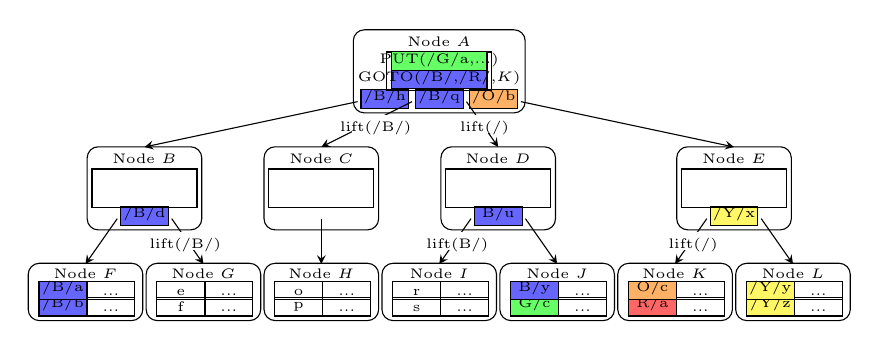
\begin{tikzpicture}[xscale=0.95, yscale=0.95]
            \node[anchor=south, rectangle, rounded corners, minimum height=.06\textwidth, minimum width=.12\textwidth, draw=black] at (0, 0) {};
            \node[anchor=south, font=\tiny] at (0, .036\textwidth) {Node $F$};
            \node[anchor=south, rectangle, minimum height=.015\textwidth, minimum width=.05\textwidth, draw=black, fill={blue!60}] at (-.025\textwidth, .005\textwidth) {};
            \node[anchor=south, font=\tiny] at (-.025\textwidth, 0) {/B/b};
            \node[anchor=south, rectangle, minimum height=.015\textwidth, minimum width=.05\textwidth, draw=black] at (.028\textwidth, .005\textwidth) {};
            \node[anchor=south, font=\tiny] at (.028\textwidth, 0) {...};
            \node[anchor=south, rectangle, minimum height=.015\textwidth, minimum width=.05\textwidth, draw=black, fill={blue!60}] at (-.025\textwidth, .023\textwidth) {};
            \node[anchor=south, font=\tiny] at (-.025\textwidth, .018\textwidth) {/B/a};
            \node[anchor=south, rectangle, minimum height=.015\textwidth, minimum width=.05\textwidth, draw=black] at (.028\textwidth, .023\textwidth) {};
            \node[anchor=south, font=\tiny] at (.028\textwidth, .018\textwidth) {...};

            \node[anchor=south, rectangle, rounded corners, minimum height=.06\textwidth, minimum width=.12\textwidth, draw=black] at (.13\textwidth, 0) {};
            \node[anchor=south, font=\tiny] at (.13\textwidth, .036\textwidth) {Node $G$};
            \node[anchor=south, rectangle, minimum height=.015\textwidth, minimum width=.05\textwidth, draw=black] at (.105\textwidth, .005\textwidth) {};
            \node[anchor=south, font=\tiny] at (.105\textwidth, 0) {f};
            \node[anchor=south, rectangle, minimum height=.015\textwidth, minimum width=.05\textwidth, draw=black] at (.158\textwidth, .005\textwidth) {};
            \node[anchor=south, font=\tiny] at (.158\textwidth, 0) {...};
            \node[anchor=south, rectangle, minimum height=.015\textwidth, minimum width=.05\textwidth, draw=black] at (.105\textwidth, .023\textwidth) {};
            \node[anchor=south, font=\tiny] at (.105\textwidth, .018\textwidth) {e};
            \node[anchor=south, rectangle, minimum height=.015\textwidth, minimum width=.05\textwidth, draw=black] at (.158\textwidth, .023\textwidth) {};
            \node[anchor=south, font=\tiny] at (.158\textwidth, .018\textwidth) {...};

            \node[anchor=south, rectangle, rounded corners, minimum height=.06\textwidth, minimum width=.12\textwidth, draw=black] at (.26\textwidth, 0) {};
            \node[anchor=south, font=\tiny] at (.26\textwidth, .036\textwidth) {Node $H$};
            \node[anchor=south, rectangle, minimum height=.015\textwidth, minimum width=.05\textwidth, draw=black] at (.235\textwidth, .005\textwidth) {};
            \node[anchor=south, font=\tiny] at (.235\textwidth, 0) {p};
            \node[anchor=south, rectangle, minimum height=.015\textwidth, minimum width=.05\textwidth, draw=black] at (.288\textwidth, .005\textwidth) {};
            \node[anchor=south, font=\tiny] at (.288\textwidth, 0) {...};
            \node[anchor=south, rectangle, minimum height=.015\textwidth, minimum width=.05\textwidth, draw=black] at (.235\textwidth, .023\textwidth) {};
            \node[anchor=south, font=\tiny] at (.235\textwidth, .018\textwidth) {o};
            \node[anchor=south, rectangle, minimum height=.015\textwidth, minimum width=.05\textwidth, draw=black] at (.288\textwidth, .023\textwidth) {};
            \node[anchor=south, font=\tiny] at (.288\textwidth, .018\textwidth) {...};

            \node[anchor=south, rectangle, rounded corners, minimum height=.06\textwidth, minimum width=.12\textwidth, draw=black] at (.39\textwidth, 0) {};
            \node[anchor=south, font=\tiny] at (.39\textwidth, .036\textwidth) {Node $I$};
            \node[anchor=south, rectangle, minimum height=.015\textwidth, minimum width=.05\textwidth, draw=black] at (.365\textwidth, .005\textwidth) {};
            \node[anchor=south, font=\tiny] at (.365\textwidth, 0) {s};
            \node[anchor=south, rectangle, minimum height=.015\textwidth, minimum width=.05\textwidth, draw=black] at (.418\textwidth, .005\textwidth) {};
            \node[anchor=south, font=\tiny] at (.418\textwidth, 0) {...};
            \node[anchor=south, rectangle, minimum height=.015\textwidth, minimum width=.05\textwidth, draw=black] at (.365\textwidth, .023\textwidth) {};
            \node[anchor=south, font=\tiny] at (.365\textwidth, .018\textwidth) {r};
            \node[anchor=south, rectangle, minimum height=.015\textwidth, minimum width=.05\textwidth, draw=black] at (.418\textwidth, .023\textwidth) {};
            \node[anchor=south, font=\tiny] at (.418\textwidth, .018\textwidth) {...};

            \node[anchor=south, rectangle, rounded corners, minimum height=.06\textwidth, minimum width=.12\textwidth, draw=black] at (.52\textwidth, 0) {};
            \node[anchor=south, font=\tiny] at (.52\textwidth, .036\textwidth) {Node $J$};
            \node[anchor=south, rectangle, minimum height=.015\textwidth, minimum width=.05\textwidth, draw=black, fill={green!60}] at (.495\textwidth, .005\textwidth) {};
            \node[anchor=south, font=\tiny] at (.495\textwidth, 0) {G/c};
            \node[anchor=south, rectangle, minimum height=.015\textwidth, minimum width=.05\textwidth, draw=black] at (.548\textwidth, .005\textwidth) {};
            \node[anchor=south, font=\tiny] at (.548\textwidth, 0) {...};
            \node[anchor=south, rectangle, minimum height=.015\textwidth, minimum width=.05\textwidth, draw=black, fill={blue!60}] at (.495\textwidth, .023\textwidth) {};
            \node[anchor=south, font=\tiny] at (.495\textwidth, .018\textwidth) {B/y};
            \node[anchor=south, rectangle, minimum height=.015\textwidth, minimum width=.05\textwidth, draw=black] at (.548\textwidth, .023\textwidth) {};
            \node[anchor=south, font=\tiny] at (.548\textwidth, .018\textwidth) {...};

            \node[anchor=south, rectangle, rounded corners, minimum height=.06\textwidth, minimum width=.12\textwidth, draw=black] at (.65\textwidth, 0) {};
            \node[anchor=south, font=\tiny] at (.65\textwidth, .036\textwidth) {Node $K$};
            \node[anchor=south, rectangle, minimum height=.015\textwidth, minimum width=.05\textwidth, draw=black, fill={red!60}] at (.625\textwidth, .005\textwidth) {};
            \node[anchor=south, font=\tiny] at (.625\textwidth, 0) {R/a};
            \node[anchor=south, rectangle, minimum height=.015\textwidth, minimum width=.05\textwidth, draw=black] at (.678\textwidth, .005\textwidth) {};
            \node[anchor=south, font=\tiny] at (.678\textwidth, 0) {...};
            \node[anchor=south, rectangle, minimum height=.015\textwidth, minimum width=.05\textwidth, draw=black, fill={orange!60}] at (.625\textwidth, .023\textwidth) {};
            \node[anchor=south, font=\tiny] at (.625\textwidth, .018\textwidth) {O/c};
            \node[anchor=south, rectangle, minimum height=.015\textwidth, minimum width=.05\textwidth, draw=black] at (.678\textwidth, .023\textwidth) {};
            \node[anchor=south, font=\tiny] at (.678\textwidth, .018\textwidth) {...};

            \node[anchor=south, rectangle, rounded corners, minimum height=.06\textwidth, minimum width=.12\textwidth, draw=black] at (.78\textwidth, 0) {};
            \node[anchor=south, font=\tiny] at (.78\textwidth, .036\textwidth) {Node $L$};
            \node[anchor=south, rectangle, minimum height=.015\textwidth, minimum width=.05\textwidth, draw=black, fill={yellow!60}] at (.755\textwidth, .005\textwidth) {};
            \node[anchor=south, font=\tiny] at (.755\textwidth, 0) {/Y/z};
            \node[anchor=south, rectangle, minimum height=.015\textwidth, minimum width=.05\textwidth, draw=black] at (.808\textwidth, .005\textwidth) {};
            \node[anchor=south, font=\tiny] at (.808\textwidth, 0) {...};
            \node[anchor=south, rectangle, minimum height=.015\textwidth, minimum width=.05\textwidth, draw=black, fill={yellow!60}] at (.755\textwidth, .023\textwidth) {};
            \node[anchor=south, font=\tiny] at (.755\textwidth, .018\textwidth) {/Y/y};
            \node[anchor=south, rectangle, minimum height=.015\textwidth, minimum width=.05\textwidth, draw=black] at (.808\textwidth, .023\textwidth) {};
            \node[anchor=south, font=\tiny] at (.808\textwidth, .018\textwidth) {...};

            \node[anchor=south, rectangle, rounded corners, minimum height=.087\textwidth, minimum width=.12\textwidth, draw=black] at (.065\textwidth, .1\textwidth) {};
            \node[anchor=south, font=\tiny] at (.065\textwidth, .163\textwidth) {Node $B$};
            \node[anchor=south, rectangle, minimum height=.015\textwidth, minimum width=.05\textwidth, draw=black, fill={blue!60}] at (.065\textwidth, .105\textwidth) {};
            \node[anchor=south, font=\tiny] at (.065\textwidth, .1\textwidth) {/B/d};
            \node[anchor=south, rectangle, minimum height=.04\textwidth, minimum width=.11\textwidth, draw=black] at (.065\textwidth, .125\textwidth) {};

            \node[anchor=south, rectangle, rounded corners, minimum height=.087\textwidth, minimum width=.12\textwidth, draw=black] at (.26\textwidth, .1\textwidth) {};
            \node[anchor=south, font=\tiny] at (.26\textwidth, .163\textwidth) {Node $C$};
            \node[anchor=south, rectangle, minimum height=.04\textwidth, minimum width=.11\textwidth, draw=black] at (.26\textwidth, .125\textwidth) {};

            \node[anchor=south, rectangle, rounded corners, minimum height=.087\textwidth, minimum width=.12\textwidth, draw=black] at (.455\textwidth, .1\textwidth) {};
            \node[anchor=south, font=\tiny] at (.455\textwidth, .163\textwidth) {Node $D$};
            \node[anchor=south, rectangle, minimum height=.015\textwidth, minimum width=.05\textwidth, draw=black, fill={blue!60}] at (.455\textwidth, .105\textwidth) {};
            \node[anchor=south, font=\tiny] at (.455\textwidth, .1\textwidth) {B/u};
            \node[anchor=south, rectangle, minimum height=.04\textwidth, minimum width=.11\textwidth, draw=black] at (.455\textwidth, .125\textwidth) {};

            \node[anchor=south, rectangle, rounded corners, minimum height=.087\textwidth, minimum width=.12\textwidth, draw=black] at (.715\textwidth, .1\textwidth) {};
            \node[anchor=south, font=\tiny] at (.715\textwidth, .163\textwidth) {Node $E$};
            \node[anchor=south, rectangle, minimum height=.015\textwidth, minimum width=.05\textwidth, draw=black, fill={yellow!60}] at (.715\textwidth, .105\textwidth) {};
            \node[anchor=south, font=\tiny] at (.715\textwidth, .1\textwidth) {/Y/x};
            \node[anchor=south, rectangle, minimum height=.04\textwidth, minimum width=.11\textwidth, draw=black] at (.715\textwidth, .125\textwidth) {};

            \node[anchor=south, rectangle, rounded corners, minimum height=.087\textwidth, minimum width=.18\textwidth, draw=black] at (.39\textwidth, .229\textwidth) {};
            \node[anchor=south, font=\tiny] at (.39\textwidth, .292\textwidth) {Node $A$};
            \node[anchor=south, rectangle, minimum height=.015\textwidth, minimum width=.05\textwidth, draw=black, fill={blue!60}] at (.33\textwidth, .234\textwidth) {};
            \node[anchor=south, font=\tiny] at (.33\textwidth, .229\textwidth) {/B/h};
            \node[anchor=south, rectangle, minimum height=.015\textwidth, minimum width=.05\textwidth, draw=black, fill={blue!60}] at (.39\textwidth, .234\textwidth) {};
            \node[anchor=south, font=\tiny] at (.39\textwidth, .229\textwidth) {/B/q};
            \node[anchor=south, rectangle, minimum height=.015\textwidth, minimum width=.05\textwidth, draw=black, fill={orange!60}] at (.45\textwidth, .234\textwidth) {};
            \node[anchor=south, font=\tiny] at (.45\textwidth, .229\textwidth) {/O/b};
            \node[anchor=south, rectangle, minimum height=.04\textwidth, minimum width=.11\textwidth, draw=black] at (.39\textwidth, .254\textwidth) {};
            \node[anchor=south, rectangle, minimum height=.015\textwidth, minimum width=.1\textwidth, draw=black, fill={blue!60}] at (.39\textwidth, .256\textwidth) {};
            \node[anchor=south, font=\tiny] at  (.39\textwidth, .25\textwidth) {GOTO(/B/,/R/,$K$)};
            \node[anchor=south, rectangle, minimum height=.015\textwidth, minimum width=.1\textwidth, draw=black, fill={green!60}] at (.39\textwidth, .276\textwidth) {};
            \node[anchor=south, font=\tiny] at  (.39\textwidth, .27\textwidth) {PUT(/G/a,...)};

            \draw[->, >=stealth] (.035\textwidth, .113\textwidth) -- (0, .063\textwidth);
            \draw[->, >=stealth] (.095\textwidth, .113\textwidth) -- (.13\textwidth, .063\textwidth);
            \draw[->, >=stealth] (.26\textwidth, .113\textwidth) -- (.26\textwidth, .063\textwidth);
            \draw[->, >=stealth] (.425\textwidth, .113\textwidth) -- (.39\textwidth, .063\textwidth);
            \draw[->, >=stealth] (.485\textwidth, .113\textwidth) -- (.52\textwidth, .063\textwidth);
            \draw[->, >=stealth] (.685\textwidth, .113\textwidth) -- (.65\textwidth, .063\textwidth);
            \draw[->, >=stealth] (.745\textwidth, .113\textwidth) -- (.78\textwidth, .063\textwidth);
            \draw[->, >=stealth] (.3\textwidth, .242\textwidth) -- (.065\textwidth, .192\textwidth);
            \draw[->, >=stealth] (.36\textwidth, .242\textwidth) -- (.26\textwidth, .192\textwidth);
            \draw[->, >=stealth] (.42\textwidth, .242\textwidth) -- (.455\textwidth, .192\textwidth);
            \draw[->, >=stealth] (.48\textwidth, .242\textwidth) -- (.715\textwidth, .192\textwidth);

            \node[anchor=north,rectangle, minimum height=.015\textwidth, minimum width=.05\textwidth, fill={white}] at (.32\textwidth, .228\textwidth) {};
            \node[anchor=north, font=\tiny] at (.32\textwidth, .231\textwidth) {lift(/B/)};
            \node[anchor=north,rectangle, minimum height=.015\textwidth, minimum width=.05\textwidth, fill={white}] at (.44\textwidth, .228\textwidth) {};
            \node[anchor=north, font=\tiny] at (.44\textwidth, .231\textwidth) {lift(/)};
            \node[anchor=north,rectangle, minimum height=.015\textwidth, minimum width=.05\textwidth, fill={white}] at (.11\textwidth, .099\textwidth) {};
            \node[anchor=north, font=\tiny] at (.11\textwidth, .102\textwidth) {lift(/B/)};
            \node[anchor=north,rectangle, minimum height=.015\textwidth, minimum width=.05\textwidth, fill={white}] at (.41\textwidth, .099\textwidth) {};
            \node[anchor=north, font=\tiny] at (.41\textwidth, .102\textwidth) {lift(B/)};
            \node[anchor=north,rectangle, minimum height=.015\textwidth, minimum width=.05\textwidth, fill={white}] at (.67\textwidth, .099\textwidth) {};
            \node[anchor=north, font=\tiny] at (.67\textwidth, .102\textwidth) {lift(/)};
        \end{tikzpicture}
        \caption{\label{subfig:flush-1} The lifted \bedag wants to flush the
            \goto message from Node $A$, however, the \goto message doesn't
            fit into any child.}
    \end{subfigure}
    \begin{subfigure}{\textwidth}
        \centering
        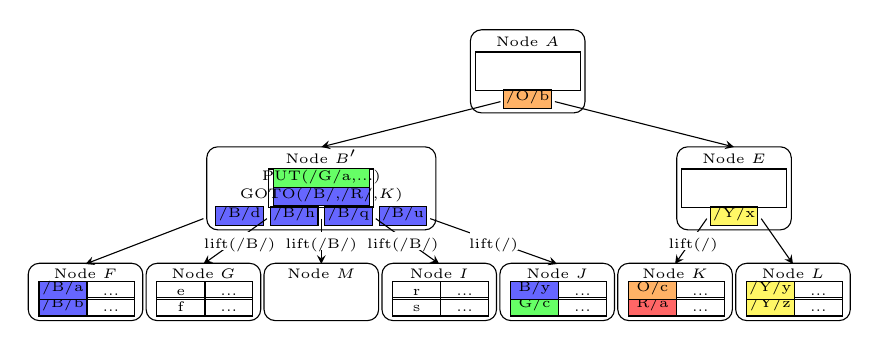
\begin{tikzpicture}[xscale=0.95, yscale=0.95]
            \node[anchor=south, rectangle, rounded corners, minimum height=.06\textwidth, minimum width=.12\textwidth, draw=black] at (0, 0) {};
            \node[anchor=south, font=\tiny] at (0, .036\textwidth) {Node $F$};
            \node[anchor=south, rectangle, minimum height=.015\textwidth, minimum width=.05\textwidth, draw=black, fill={blue!60}] at (-.025\textwidth, .005\textwidth) {};
            \node[anchor=south, font=\tiny] at (-.025\textwidth, 0) {/B/b};
            \node[anchor=south, rectangle, minimum height=.015\textwidth, minimum width=.05\textwidth, draw=black] at (.028\textwidth, .005\textwidth) {};
            \node[anchor=south, font=\tiny] at (.028\textwidth, 0) {...};
            \node[anchor=south, rectangle, minimum height=.015\textwidth, minimum width=.05\textwidth, draw=black, fill={blue!60}] at (-.025\textwidth, .023\textwidth) {};
            \node[anchor=south, font=\tiny] at (-.025\textwidth, .018\textwidth) {/B/a};
            \node[anchor=south, rectangle, minimum height=.015\textwidth, minimum width=.05\textwidth, draw=black] at (.028\textwidth, .023\textwidth) {};
            \node[anchor=south, font=\tiny] at (.028\textwidth, .018\textwidth) {...};

            \node[anchor=south, rectangle, rounded corners, minimum height=.06\textwidth, minimum width=.12\textwidth, draw=black] at (.13\textwidth, 0) {};
            \node[anchor=south, font=\tiny] at (.13\textwidth, .036\textwidth) {Node $G$};
            \node[anchor=south, rectangle, minimum height=.015\textwidth, minimum width=.05\textwidth, draw=black] at (.105\textwidth, .005\textwidth) {};
            \node[anchor=south, font=\tiny] at (.105\textwidth, 0) {f};
            \node[anchor=south, rectangle, minimum height=.015\textwidth, minimum width=.05\textwidth, draw=black] at (.158\textwidth, .005\textwidth) {};
            \node[anchor=south, font=\tiny] at (.158\textwidth, 0) {...};
            \node[anchor=south, rectangle, minimum height=.015\textwidth, minimum width=.05\textwidth, draw=black] at (.105\textwidth, .023\textwidth) {};
            \node[anchor=south, font=\tiny] at (.105\textwidth, .018\textwidth) {e};
            \node[anchor=south, rectangle, minimum height=.015\textwidth, minimum width=.05\textwidth, draw=black] at (.158\textwidth, .023\textwidth) {};
            \node[anchor=south, font=\tiny] at (.158\textwidth, .018\textwidth) {...};

            \node[anchor=south, rectangle, rounded corners, minimum height=.06\textwidth, minimum width=.12\textwidth, draw=black] at (.26\textwidth, 0) {};
            \node[anchor=south, font=\tiny] at (.26\textwidth, .036\textwidth) {Node $M$};

            \node[anchor=south, rectangle, rounded corners, minimum height=.06\textwidth, minimum width=.12\textwidth, draw=black] at (.39\textwidth, 0) {};
            \node[anchor=south, font=\tiny] at (.39\textwidth, .036\textwidth) {Node $I$};
            \node[anchor=south, rectangle, minimum height=.015\textwidth, minimum width=.05\textwidth, draw=black] at (.365\textwidth, .005\textwidth) {};
            \node[anchor=south, font=\tiny] at (.365\textwidth, 0) {s};
            \node[anchor=south, rectangle, minimum height=.015\textwidth, minimum width=.05\textwidth, draw=black] at (.418\textwidth, .005\textwidth) {};
            \node[anchor=south, font=\tiny] at (.418\textwidth, 0) {...};
            \node[anchor=south, rectangle, minimum height=.015\textwidth, minimum width=.05\textwidth, draw=black] at (.365\textwidth, .023\textwidth) {};
            \node[anchor=south, font=\tiny] at (.365\textwidth, .018\textwidth) {r};
            \node[anchor=south, rectangle, minimum height=.015\textwidth, minimum width=.05\textwidth, draw=black] at (.418\textwidth, .023\textwidth) {};
            \node[anchor=south, font=\tiny] at (.418\textwidth, .018\textwidth) {...};

            \node[anchor=south, rectangle, rounded corners, minimum height=.06\textwidth, minimum width=.12\textwidth, draw=black] at (.52\textwidth, 0) {};
            \node[anchor=south, font=\tiny] at (.52\textwidth, .036\textwidth) {Node $J$};
            \node[anchor=south, rectangle, minimum height=.015\textwidth, minimum width=.05\textwidth, draw=black, fill={green!60}] at (.495\textwidth, .005\textwidth) {};
            \node[anchor=south, font=\tiny] at (.495\textwidth, 0) {G/c};
            \node[anchor=south, rectangle, minimum height=.015\textwidth, minimum width=.05\textwidth, draw=black] at (.548\textwidth, .005\textwidth) {};
            \node[anchor=south, font=\tiny] at (.548\textwidth, 0) {...};
            \node[anchor=south, rectangle, minimum height=.015\textwidth, minimum width=.05\textwidth, draw=black, fill={blue!60}] at (.495\textwidth, .023\textwidth) {};
            \node[anchor=south, font=\tiny] at (.495\textwidth, .018\textwidth) {B/y};
            \node[anchor=south, rectangle, minimum height=.015\textwidth, minimum width=.05\textwidth, draw=black] at (.548\textwidth, .023\textwidth) {};
            \node[anchor=south, font=\tiny] at (.548\textwidth, .018\textwidth) {...};

            \node[anchor=south, rectangle, rounded corners, minimum height=.06\textwidth, minimum width=.12\textwidth, draw=black] at (.65\textwidth, 0) {};
            \node[anchor=south, font=\tiny] at (.65\textwidth, .036\textwidth) {Node $K$};
            \node[anchor=south, rectangle, minimum height=.015\textwidth, minimum width=.05\textwidth, draw=black, fill={red!60}] at (.625\textwidth, .005\textwidth) {};
            \node[anchor=south, font=\tiny] at (.625\textwidth, 0) {R/a};
            \node[anchor=south, rectangle, minimum height=.015\textwidth, minimum width=.05\textwidth, draw=black] at (.678\textwidth, .005\textwidth) {};
            \node[anchor=south, font=\tiny] at (.678\textwidth, 0) {...};
            \node[anchor=south, rectangle, minimum height=.015\textwidth, minimum width=.05\textwidth, draw=black, fill={orange!60}] at (.625\textwidth, .023\textwidth) {};
            \node[anchor=south, font=\tiny] at (.625\textwidth, .018\textwidth) {O/c};
            \node[anchor=south, rectangle, minimum height=.015\textwidth, minimum width=.05\textwidth, draw=black] at (.678\textwidth, .023\textwidth) {};
            \node[anchor=south, font=\tiny] at (.678\textwidth, .018\textwidth) {...};

            \node[anchor=south, rectangle, rounded corners, minimum height=.06\textwidth, minimum width=.12\textwidth, draw=black] at (.78\textwidth, 0) {};
            \node[anchor=south, font=\tiny] at (.78\textwidth, .036\textwidth) {Node $L$};
            \node[anchor=south, rectangle, minimum height=.015\textwidth, minimum width=.05\textwidth, draw=black, fill={yellow!60}] at (.755\textwidth, .005\textwidth) {};
            \node[anchor=south, font=\tiny] at (.755\textwidth, 0) {/Y/z};
            \node[anchor=south, rectangle, minimum height=.015\textwidth, minimum width=.05\textwidth, draw=black] at (.808\textwidth, .005\textwidth) {};
            \node[anchor=south, font=\tiny] at (.808\textwidth, 0) {...};
            \node[anchor=south, rectangle, minimum height=.015\textwidth, minimum width=.05\textwidth, draw=black, fill={yellow!60}] at (.755\textwidth, .023\textwidth) {};
            \node[anchor=south, font=\tiny] at (.755\textwidth, .018\textwidth) {/Y/y};
            \node[anchor=south, rectangle, minimum height=.015\textwidth, minimum width=.05\textwidth, draw=black] at (.808\textwidth, .023\textwidth) {};
            \node[anchor=south, font=\tiny] at (.808\textwidth, .018\textwidth) {...};

            \node[anchor=south, rectangle, rounded corners, minimum height=.087\textwidth, minimum width=.24\textwidth, draw=black] at (.26\textwidth, .1\textwidth) {};
            \node[anchor=south, font=\tiny] at (.26\textwidth, .163\textwidth) {Node $B'$};
            \node[anchor=south, rectangle, minimum height=.015\textwidth, minimum width=.05\textwidth, draw=black, fill={blue!60}] at (.17\textwidth, .105\textwidth) {};
            \node[anchor=south, font=\tiny] at (.17\textwidth, .1\textwidth) {/B/d};
            \node[anchor=south, rectangle, minimum height=.015\textwidth, minimum width=.05\textwidth, draw=black, fill={blue!60}] at (.23\textwidth, .105\textwidth) {};
            \node[anchor=south, font=\tiny] at (.23\textwidth, .1\textwidth) {/B/h};
            \node[anchor=south, rectangle, minimum height=.015\textwidth, minimum width=.05\textwidth, draw=black, fill={blue!60}] at (.29\textwidth, .105\textwidth) {};
            \node[anchor=south, font=\tiny] at (.29\textwidth, .1\textwidth) {/B/q};
            \node[anchor=south, rectangle, minimum height=.015\textwidth, minimum width=.05\textwidth, draw=black, fill={blue!60}] at (.35\textwidth, .105\textwidth) {};
            \node[anchor=south, font=\tiny] at (.35\textwidth, .1\textwidth) {/B/u};
            \node[anchor=south, rectangle, minimum height=.04\textwidth, minimum width=.11\textwidth, draw=black] at (.26\textwidth, .125\textwidth) {};
            \node[anchor=south, rectangle, minimum height=.015\textwidth, minimum width=.1\textwidth, draw=black, fill={blue!60}] at (.26\textwidth, .127\textwidth) {};
            \node[anchor=south, font=\tiny] at  (.26\textwidth, .121\textwidth) {GOTO(/B/,/R/,$K$)};
            \node[anchor=south, rectangle, minimum height=.015\textwidth, minimum width=.1\textwidth, draw=black, fill={green!60}] at (.26\textwidth, .147\textwidth) {};
            \node[anchor=south, font=\tiny] at  (.26\textwidth, .141\textwidth) {PUT(/G/a,...)};

            \node[anchor=south, rectangle, rounded corners, minimum height=.087\textwidth, minimum width=.12\textwidth, draw=black] at (.715\textwidth, .1\textwidth) {};
            \node[anchor=south, font=\tiny] at (.715\textwidth, .163\textwidth) {Node $E$};
            \node[anchor=south, rectangle, minimum height=.015\textwidth, minimum width=.05\textwidth, draw=black, fill={yellow!60}] at (.715\textwidth, .105\textwidth) {};
            \node[anchor=south, font=\tiny] at (.715\textwidth, .1\textwidth) {/Y/x};
            \node[anchor=south, rectangle, minimum height=.04\textwidth, minimum width=.11\textwidth, draw=black] at (.715\textwidth, .125\textwidth) {};

            \node[anchor=south, rectangle, rounded corners, minimum height=.087\textwidth, minimum width=.12\textwidth, draw=black] at (.4875\textwidth, .229\textwidth) {};
            \node[anchor=south, font=\tiny] at (.4875\textwidth, .292\textwidth) {Node $A$};
            \node[anchor=south, rectangle, minimum height=.015\textwidth, minimum width=.05\textwidth, draw=black, fill={orange!60}] at (.4875\textwidth, .234\textwidth) {};
            \node[anchor=south, font=\tiny] at (.4875\textwidth, .229\textwidth) {/O/b};
            \node[anchor=south, rectangle, minimum height=.04\textwidth, minimum width=.11\textwidth, draw=black] at (.4875\textwidth, .254\textwidth) {};

            \draw[->, >=stealth] (.13\textwidth, .113\textwidth) -- (0, .063\textwidth);
            \draw[->, >=stealth] (.20\textwidth, .113\textwidth) -- (.13\textwidth, .063\textwidth);
            \draw[->, >=stealth] (.26\textwidth, .113\textwidth) -- (.26\textwidth, .063\textwidth);
            \draw[->, >=stealth] (.32\textwidth, .113\textwidth) -- (.39\textwidth, .063\textwidth);
            \draw[->, >=stealth] (.38\textwidth, .113\textwidth) -- (.52\textwidth, .063\textwidth);
            \draw[->, >=stealth] (.685\textwidth, .113\textwidth) -- (.65\textwidth, .063\textwidth);
            \draw[->, >=stealth] (.745\textwidth, .113\textwidth) -- (.78\textwidth, .063\textwidth);
            \draw[->, >=stealth] (.4575\textwidth, .242\textwidth) -- (.26\textwidth, .192\textwidth);
            \draw[->, >=stealth] (.5175\textwidth, .242\textwidth) -- (.715\textwidth, .192\textwidth);

            \node[anchor=north,rectangle, minimum height=.015\textwidth, minimum width=.05\textwidth, fill={white}] at (.17\textwidth, .099\textwidth) {};
            \node[anchor=north, font=\tiny] at (.17\textwidth, .102\textwidth) {lift(/B/)};
            \node[anchor=north,rectangle, minimum height=.015\textwidth, minimum width=.05\textwidth, fill={white}] at (.26\textwidth, .099\textwidth) {};
            \node[anchor=north, font=\tiny] at (.26\textwidth, .102\textwidth) {lift(/B/)};
            \node[anchor=north,rectangle, minimum height=.015\textwidth, minimum width=.05\textwidth, fill={white}] at (.35\textwidth, .099\textwidth) {};
            \node[anchor=north, font=\tiny] at (.35\textwidth, .102\textwidth) {lift(/B/)};
            \node[anchor=north,rectangle, minimum height=.015\textwidth, minimum width=.05\textwidth, fill={white}] at (.45\textwidth, .099\textwidth) {};
            \node[anchor=north, font=\tiny] at (.45\textwidth, .102\textwidth) {lift(/)};
            \node[anchor=north,rectangle, minimum height=.015\textwidth, minimum width=.05\textwidth, fill={white}] at (.67\textwidth, .099\textwidth) {};
            \node[anchor=north, font=\tiny] at (.67\textwidth, .102\textwidth) {lift(/)};
        \end{tikzpicture}
        \caption{\label{subfig:flush-2} The lifted \bedag discards Node $C$ and
            merges Node $B$ and $D$ into Node $B'$, which can accommodate the
            \goto message.}
    \end{subfigure}
    \caption[An example of flushing \goto messages merges children]{\label{fig:flush}
        The \bedag may need to merge children before flushing}
\end{figure}

When a non-leaf node fills, the lifted \bedag flushes messages, including \goto
messages, to one or more children.
In the simple case, the node for a \goto message has a single child that covers
the key range of the \goto message, $(\dpre_{min}, \dpre_{max})$.
In this case, flushing the \goto simply lifts the \dpre in the messages and
moves the message from a parent to child buffer,
provided the \goto has not yet reached its target height.

In the more complicated case, a \goto message can overlap with multiple
children.
There are fringe children whose key ranges are partly covered by the \goto
message, and partly out of the \goto range;
there are also some interior children between fringe children that are entirely
within the key range occluded by the \goto.
The lift \bedag needs to create a single child that can accommodate the \goto
message.

To this end, the \bedag simply removes the references and pointers to the
interior children (potentially garbage collecting these nodes later, if this is
the last reference),
and merges the two fringe children into one node.

Figure~\ref{fig:flush} shows an example of merging children before flushing a
\goto message.
In Figure~\ref{subfig:flush-1}, Node $B$, $C$ and $D$ all overlaps with the
range of the \goto message.
Node $B$ AND $D$ are fringe children, while Node $C$ is an interior child.
To flush the \goto message, in Figure~\ref{subfig:flush-2}, the lifted \bedag
sends Node $C$ to the background garbage collection thread and merges Node $B$
and $D$ into Node $B'$.
Note, this merge needs to create an empty node, Node Z, to cover the range
(``/B/h'', ``/B/q'').
With key lifting, changing the range of a node needs to re-lift the node.
Therefore, in order to keep Node $E$, $F$, $G$ and $H$ untouched, the merge
adds an empty node for the range not covered by those nodes.

As shown in the example, discarding interior children creates a key range that
is not covered by the fringe children.
Therefore, there will be a key range that is not covered by the children of the
node generated by the merge.
With key lift, it is not easy to change the key range of a node.
The problem is solved by adding an empty subtree for that key range as a child
of the generated node.

\paragraph{Converting \goto messages to pivots and parent-to-child pointers.}
When the lifted \bedag tries to flush a \goto message from a node that is one
level higher than the source LCA of the \goto messages, it coverts the \goto
message into two pivots and a parent-to-child pointer in the node.
This ensures a bounded depth for any root-to-leaf traversal.

This is done by adding \dpre$_{min}$ and \dpre$_{max}$ as two new pivots and
set the parent-to-child pointer to the source LCA of the \goto message.
Assume \dpre$_{min}$ and \dpre$_{max}$ are in the range of child $i$ of the node
(the lifted \bedag can perform a aforementioned merge to generate such a child),
i.e., $\dpre_{min}, \dpre_{max} \in (pivot_{i},pivot_{i+1})$.
Adding \dpre$_{min}$ and \dpre$_{max}$ as two new pivots creates 3 key ranges,
$(pivot_{i},\dpre_{min})$, $(\dpre_{min},\dpre_{max})$ and
$(\dpre_{max}, pivot_{i+1})$.
Key range $(\dpre_{min},\dpre_{max})$ is cover in the source LCA of the \goto
message, while the other two are covered by child $i$.

However, all three parent-to-child pointers now points to a child whose key
range is different than those specified in the node.
In particular, child $i$ has range $(pivot_{i},pivot_{i+1})$ but bounded by
$(pivot_{i},\dpre_{min})$ or $(\dpre_{max}, pivot_{i+1})$.
A smaller key range may lifts longer prefixes through the parent-to-child
pointer.
The source LCA has a key range that might be larger than
$(\spre_{min}, \spre_{max})$ but bounded by $(\dpre_{min},\dpre_{max})$.

The problem is solved by augmenting parent-to-child pointers with \xf functions.
Each parent-to-child pointer now has a \xf function with a prefix.
After the query lifts its search key by the LCP of two pivots, the \xf function
prepends its prefix to the search key.
Also, \xf functions serves as filters, queries need to remember the key range
specified by the pivots in the parent so that it can ignore invalid keys in the
child.

\begin{figure}
    \begin{subfigure}{\textwidth}
        \centering
        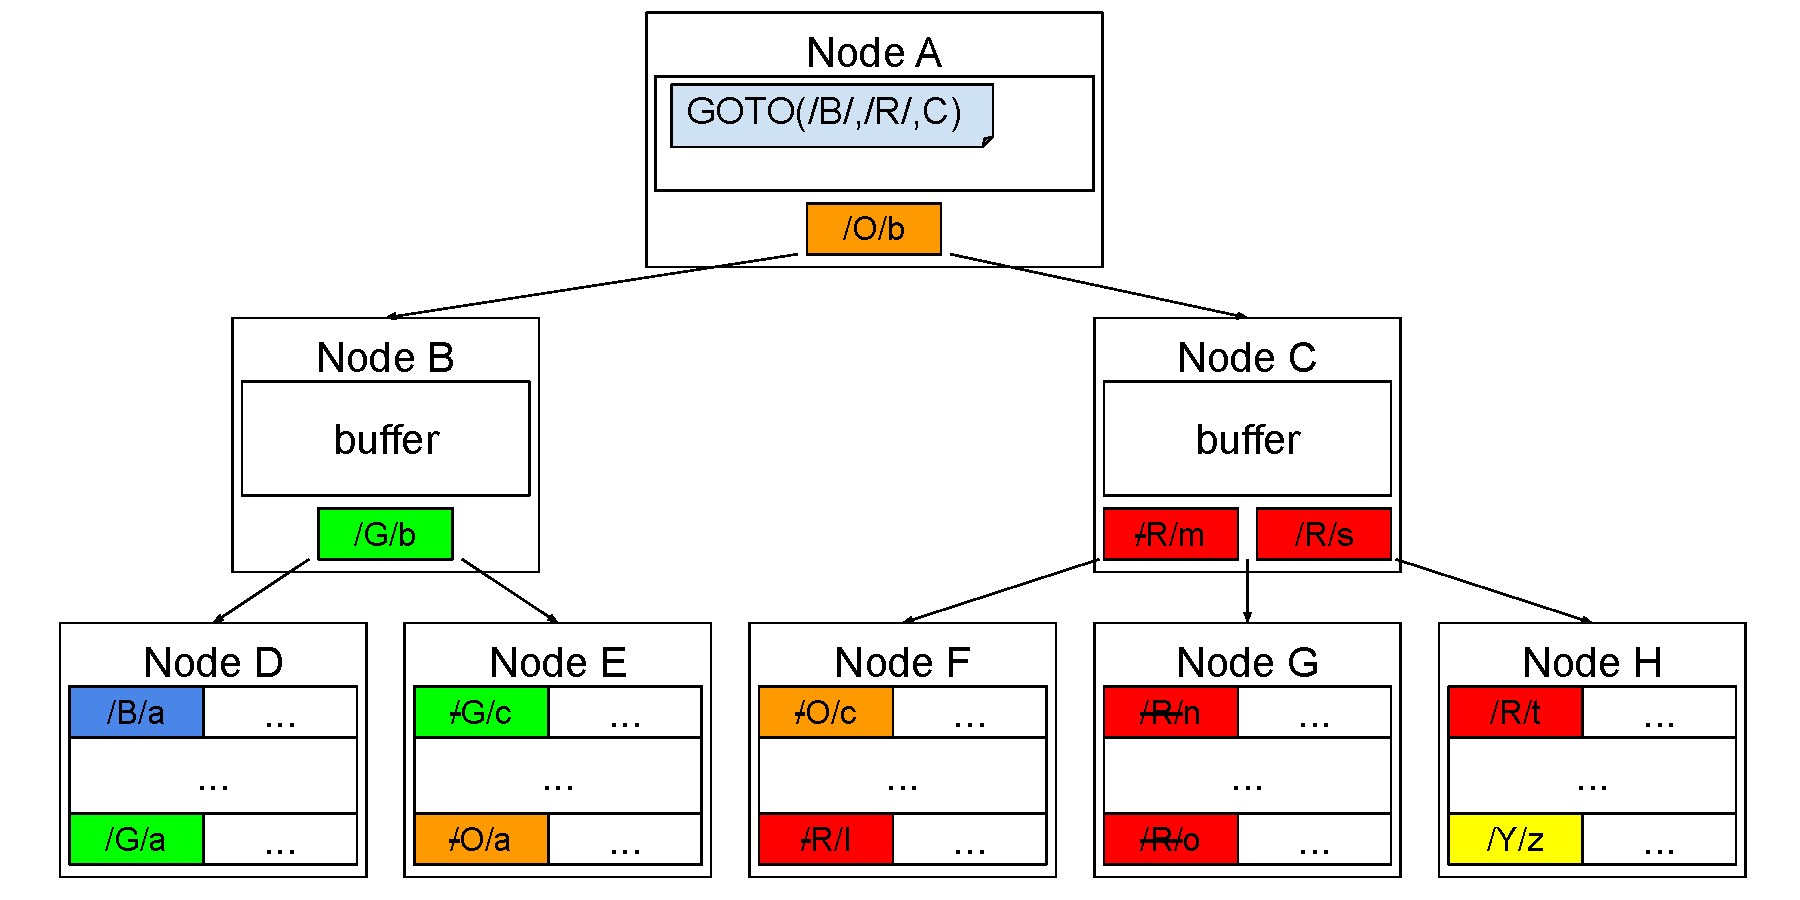
\includegraphics[width=.9\linewidth]{fig/goto-2}
        \caption{\label{subfig:spvt-1} The \goto message cannot be flushed to
            Node $B$, which is at the same as Node $C$.}
    \end{subfigure}
    \begin{subfigure}{\textwidth}
        \centering
        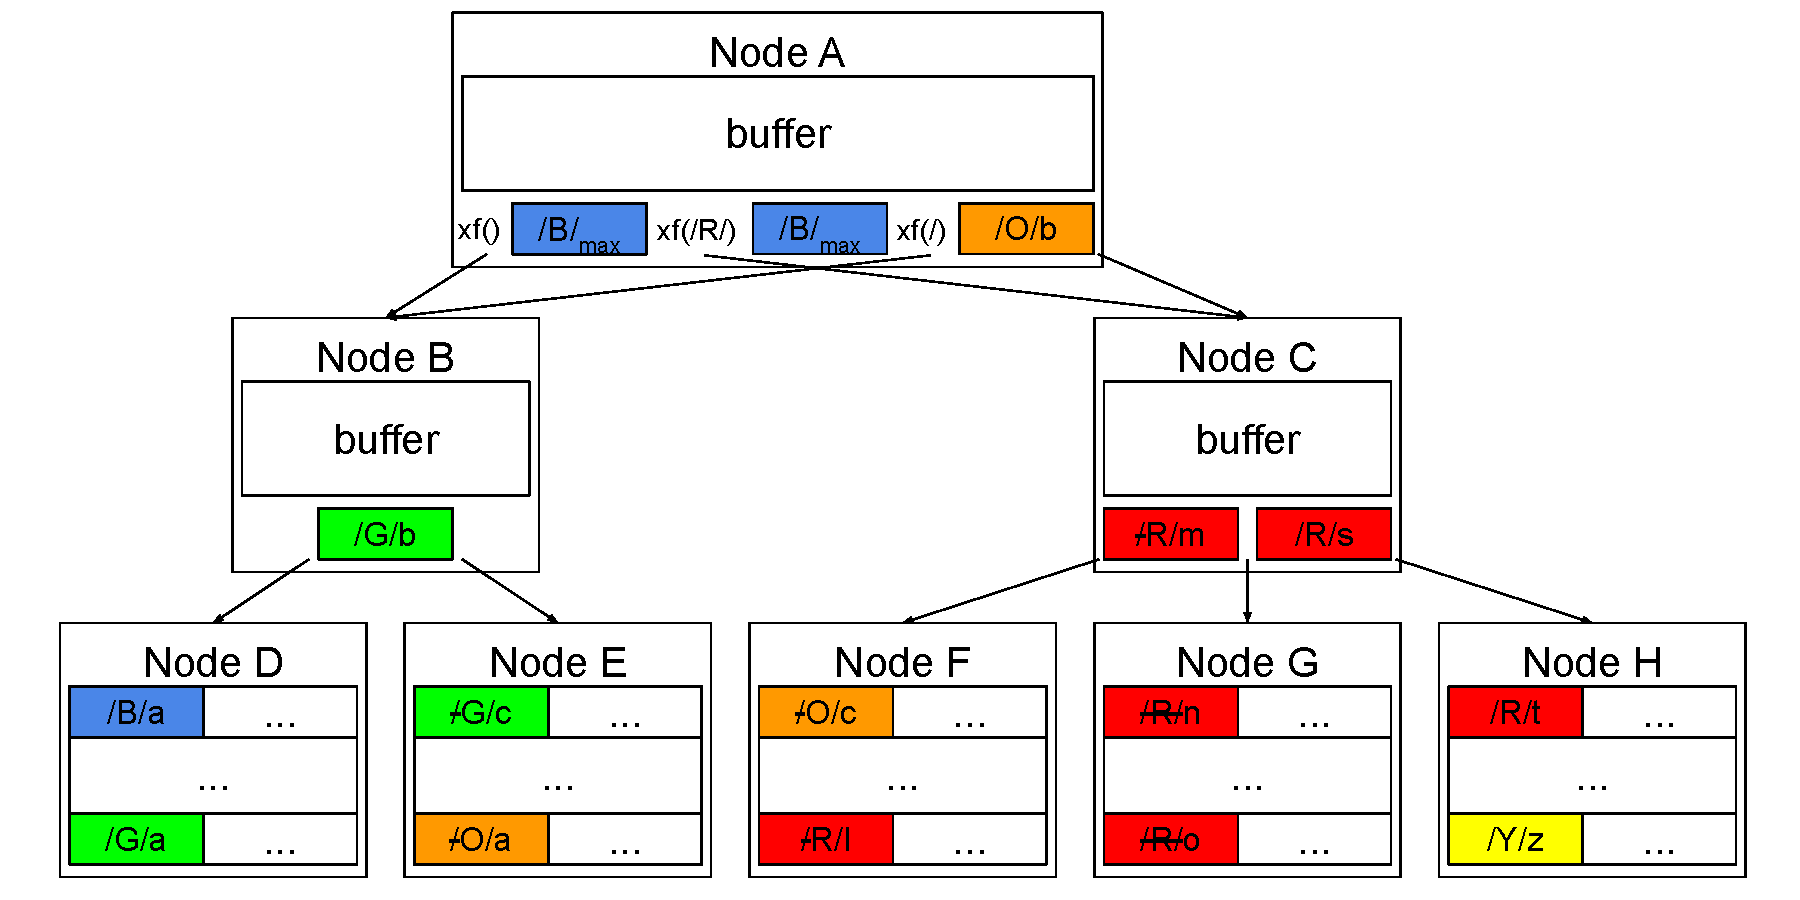
\includegraphics[width=.9\linewidth]{fig/spvt-2}
        \caption{\label{subfig:spvt-2} The \goto message becomes pivots and
            adds \xf functions to parent-to-child pointers}
    \end{subfigure}
    \caption[Transform a \goto message into pivots]{\label{fig:spvt}
        When the lifted \bedag cannot flush a \goto message deeper, it
        transforms the \goto message into pivots and adds \xf functions to
        parent-to-child pointers.}
\end{figure}

Figure~\ref{fig:spvt} shows an example of the transformation.
The lifted \bedag cannot flush the \goto message to Node $B$, because Node $B$
is at the same height as its source LCA, Node $C$.
Therefore, it adds two pivots, ``/B/$_{min}$'' and ``/B/$_{max}$''.
The parent-to-child pointer between ``/B/$_{min}$'' and ``/B/$_{max}$'' points
to the source LCA, Node $C$, and has a \xf function of ``/R/'', indicating a
key range mismatch and addition prefix ``/R/'' in the child.
Queries following that parent-to-child pointer should prepend prefix ``/R/''
after the normal lifting of ``/B/'' from its search key.
Also, they remember only keys between ``/R/$_{min}$'' and ``/R/$_{max}$'' in
the child are valid.
Similarly, two \xf functions are added to the other two pointers.
Note, for the leftmost pointer, though the \xf function contains no prefix,
it still serves as a filter for queries.

\paragraph{Fix \xf functions in parent-to-child pointers.}
\goto messages adds \xf functions to parent-to-child pointers, which indicates
the child has a larger key range and keys in the child have additional prefixes.

Before flushing to a node, if the pointer has a \xf function, the
lifted \bedag propagates the \xf function to pointers of the node.
Specifically, the lifted \bedag first discards all exterior children of the node
whose key ranges are completely out of that indicated by the \xf function.
Then, it removes the prefix in the \xf function from those keys.
At last, for fringe children whose key ranges partly overlap with that indicated
by the \xf function, it adds \xf functions to the pointers to those children.

\begin{figure}
    \begin{subfigure}{\textwidth}
        \centering
        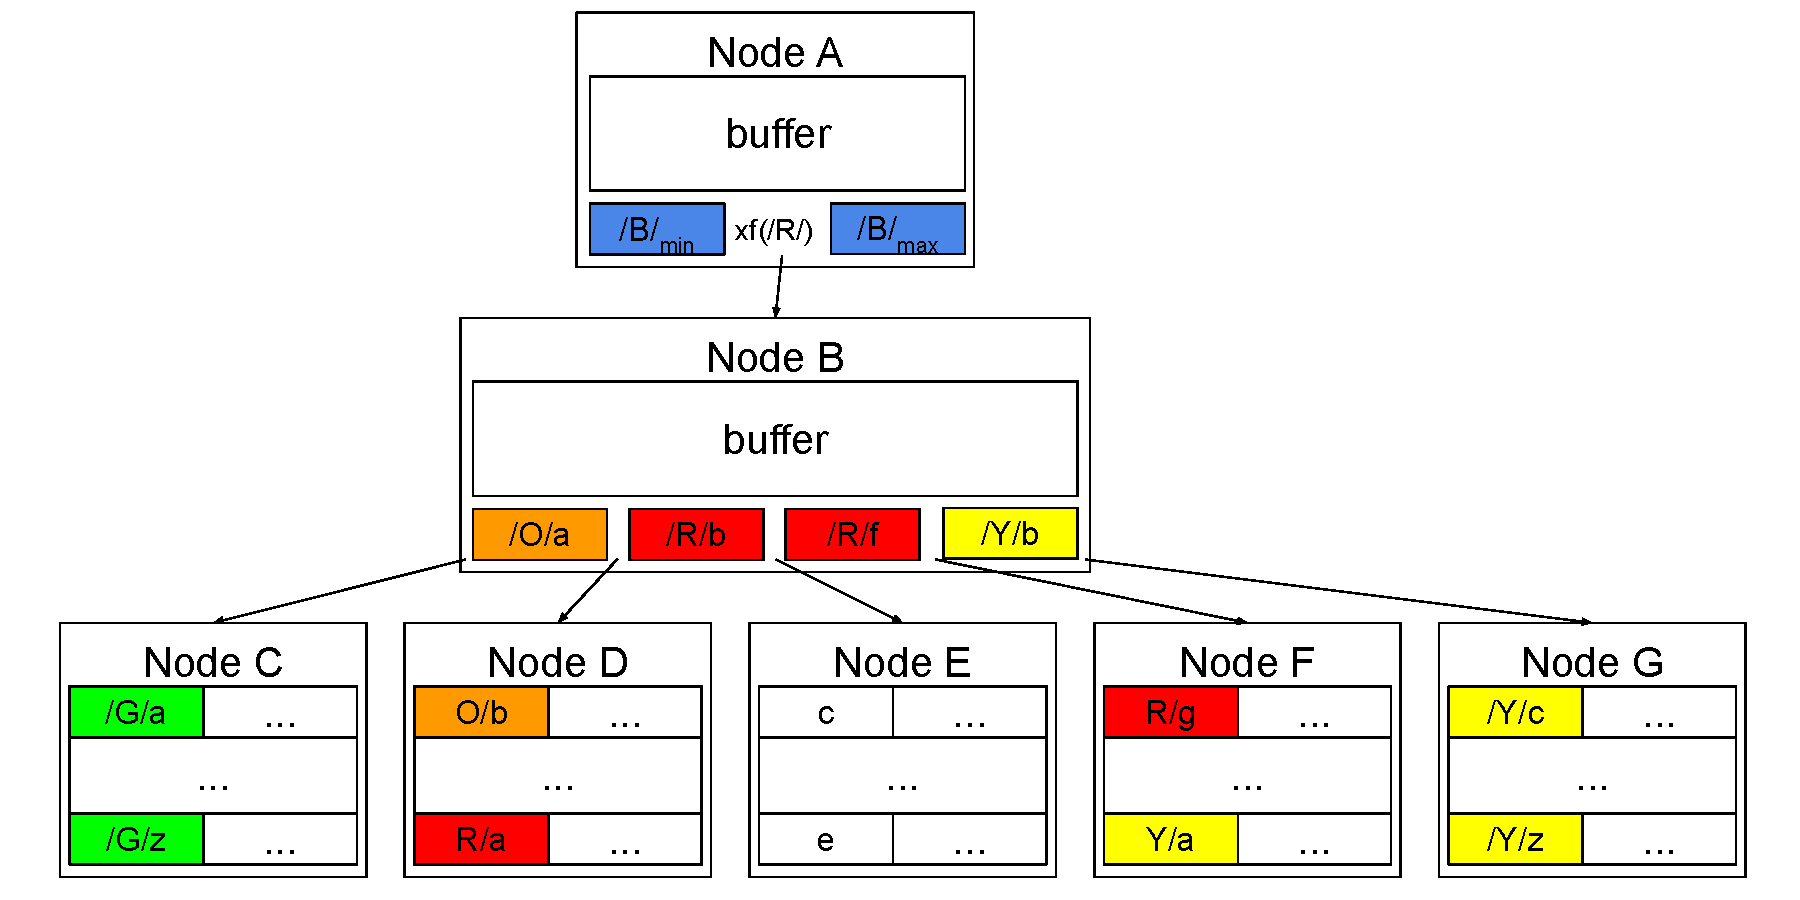
\includegraphics[width=.9\linewidth]{fig/xf-1}
        \caption{\label{subfig:xf-1} The parent-to-child pointer from Node $A$
            to Node $B$ has \xf(``/R/'').}
    \end{subfigure}
    \begin{subfigure}{\textwidth}
        \centering
        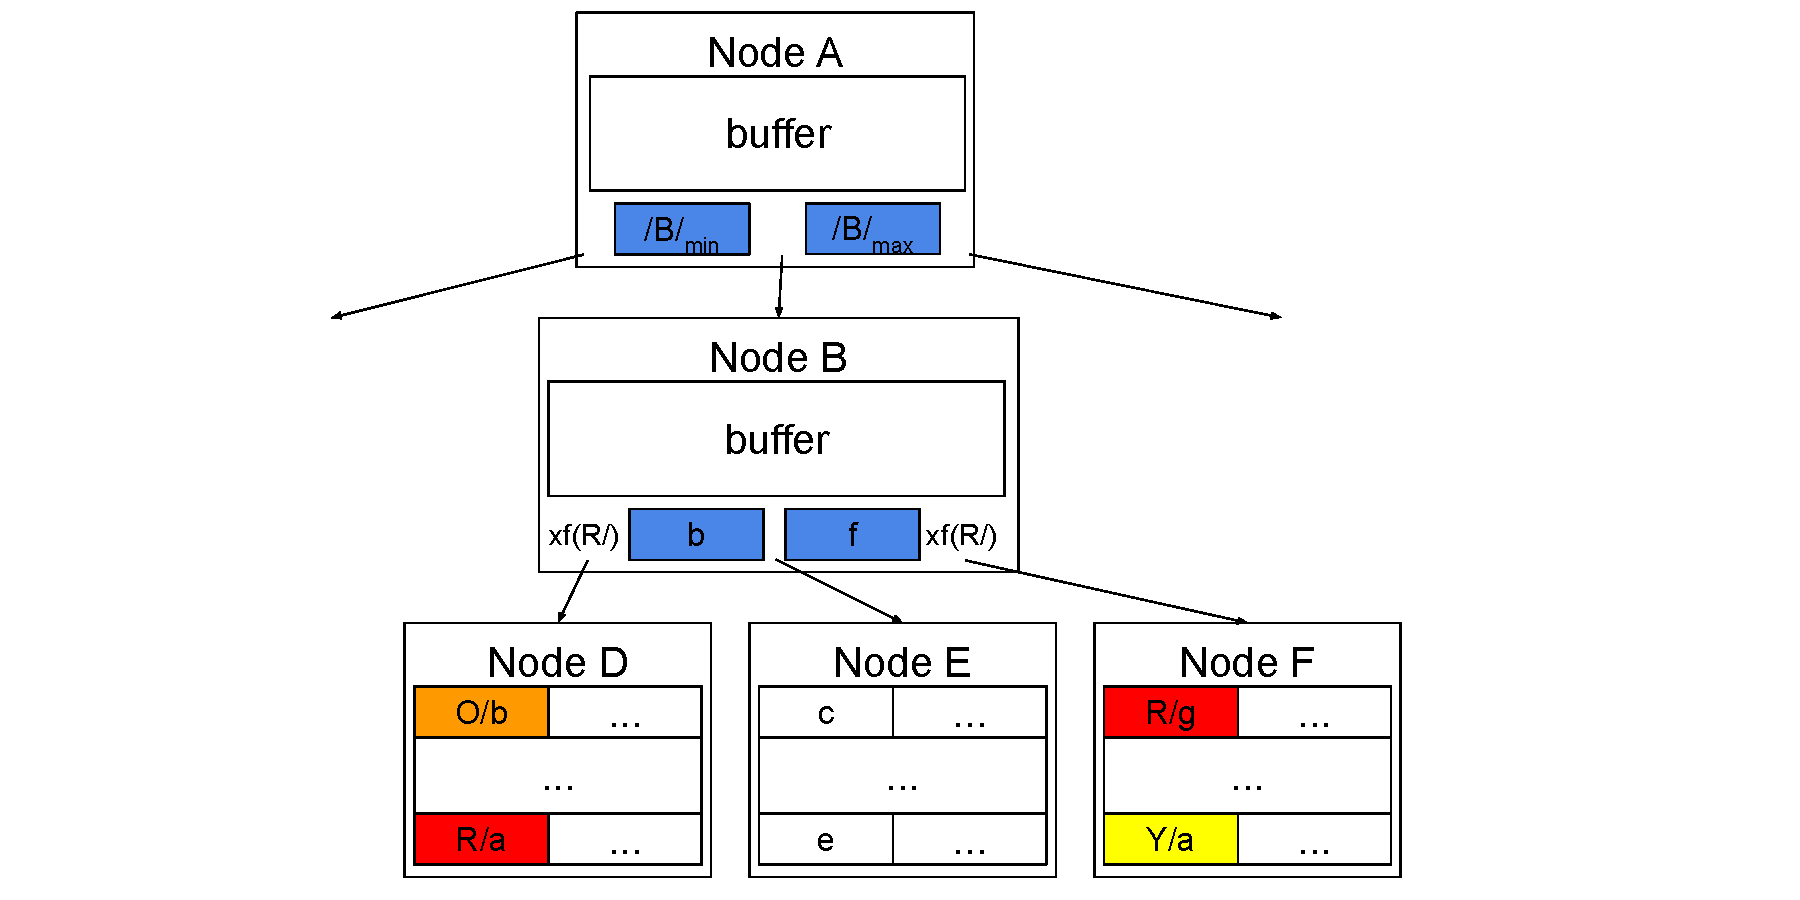
\includegraphics[width=.9\linewidth]{fig/xf-2}
        \caption{\label{subfig:xf-2} To remove the \xf function, it discards
            exterior children and adds \xf functions to parent-to-child pointers
            of fringe children.}
    \end{subfigure}
    \caption[Fix a \xf function during flushing]{\label{fig:xf}
        Before flushing messages to a node, the lifted \bedag fixes the \xf
        function associated with the parent-to-child pointer.}
\end{figure}

Figure~\ref{fig:xf} shows an example of fixing \xf functions before flushing.
In Figure~\ref{subfig:xf-2}, exterior nodes, Node $C$ and $G$ out are discarded.
Then, it adds \xf functions to pointers to fringe nodes, Node $D$ and $F$.
At last, it updates keys in Node $B$ by removing the prefix in the \xf function.

\section{Preferential splitting}

Most of the additional background work in range-clone is about removing
unrelated keys and unlifted prefix data from fringe nodes, which
contain both cloned and non-cloned data.
Therefore, it is beneficial to reduce the number of fringe nodes.

The baseline \bet splits nodes evenly.
When a leaf needs to be split, the middle key is picked as the new piovt
separating the two new leaves to be generated.
A non-leaf node split can be viewed as promoting the middle pivot in the node to
the parent.

Preferential splitting generates pivots that maximizes the common prefix under
the leaf, subject to the constraint that both leaves should be at least 1/4
full.
This strategy reduces the likelihood of having fringe nodes
in a range-clone and bounds the how unbalanced leaves can be.

A naive approach would compare all keys in the range of [1/4, 3/4] of the leaf
and picking the pair of two adjacent keys that share the shortest common prefix.
But this scan can be costly.

Preferential splitting only requires the reading of two keys.
Because the shortest common prefix of adjacent keys is the same as the common
prefix of the smallest (at 1/4 of the leaf) candidate key, $k_{s}$ and
the largest (at 3/4 of the leaf) candidate key, $k_{l}$,
a good pivot can be constructed from these two keys.
In particular, preferential splitting generates a pivot that is maximum key with
prefix $p_{s}$, where $p_{s}$ that is the shortest prefix of $k_{s}$ that
contains the LCP of $k_{s}$ and $k_{l}$ and has a slash or a end-of-string as
the last character.

\section{Summary}

This chapter first describes the new interface, range-clone, that enables file
or directory renames and clones in \betrfs.
Then, it presents a range-clone implementation that finishes all works
on the critical path and transforms a lifted \bet to a lifted \bedag.
Later, it introduces \goto messages that delay tree surgery in the range-clone,
fit the implementation into the write-optimized framework of the data structure.
At last, it describes preferential splitting that reduces work needed in
tree surgery.
